\documentclass[12pt,a4paper,titlepage,twoside]{report}
\usepackage[T1]{fontenc}
\usepackage[english, spanish]{babel}
\usepackage[utf8]{inputenc}
\usepackage[style=spanish]{csquotes}

%Latin modern font
\usepackage{lmodern}

%\usepackage[backend=bibtex]{biblatex}
%\bibliography{bibliografia.bib} % or

\usepackage{hyperref}
\usepackage{bookmark}
\usepackage[numbers]{natbib}

\usepackage{graphicx}
% Con esta opción no cargo las imágenes sólo sus espacios
%\usepackage[draft]{graphicx}
\usepackage{wrapfig} %Las imágenes quedan rodeadas de texto

%Interlineado
\usepackage{setspace}

% Parámetro para poder usar los colorines
\usepackage[pdftex,usenames,dvipsnames]{xcolor}

%Paquete para justificar el texto
\usepackage{ragged2e} 
\usepackage{notoccite}

% Penalizo la finalización o el inicio de la página con 
% lineas huerfanas
%\clubpenalty=10000
%\widowpenalty=10000

\usepackage[nottoc,numbib]{tocbibind}
\usepackage[toc,page]{appendix}

%Fancy chapter
\usepackage{titlesec, blindtext, color}
\definecolor{gray75}{gray}{0.75}
\newcommand{\hsp}{\hspace{20pt}}
\newcommand{\hsc}{\hspace{10pt}}
\titleformat{\chapter}[hang]{\LARGE\bfseries}{\thechapter\hsp\textcolor{RubineRed}{|}\hsp}{0pt}{\LARGE\bfseries}
\titleformat{\section}{\large\bfseries}{\thesection.\hsc{|}}{10pt}{\large\bfseries}


\usepackage{listings}
\usepackage{courier}
\usepackage{caption}

\lstdefinestyle{dicom}{
    basicstyle=\footnotesize\ttfamily, 
    numbers=left,              
    extendedchars=true,
    stepnumber=1,               
    captionpos=b,
    numberstyle=\tiny\color{RubineRed},
    language=XML,
    numbersep=5pt,  
    tabsize=2,                  
    extendedchars=true,         
    breaklines=true,            
    stringstyle=\color{white}\ttfamily,
    showspaces=false,           
    showtabs=false,             
    xleftmargin=5pt,
    framexleftmargin=5pt,
    framexrightmargin=5pt,
    framexbottommargin=4pt,
    %frame=single,
    backgroundcolor=\color{lightgray},
    showstringspaces=false    
}

\DeclareCaptionFont{white}{\color{white}}
\DeclareCaptionFormat{listing}{\colorbox{RubineRed}{\parbox{\textwidth}{\hspace{15pt}#1#2#3}}}
\captionsetup[lstlisting]{format=listing,labelfont=white,textfont=white, singlelinecheck=false, margin=0pt, font={bf,footnotesize}}


% Table of contents on the begining of a line. 
\usepackage{titletoc}
% Referencias
\usepackage{hyperref}

\usepackage[includefoot]{geometry}
\geometry{
  top=2cm,
  inner=2.7cm,
  outer=2.7cm,
  bottom=4cm,
  headheight=5ex,       % <-- and this
  headsep=5ex,
  footskip = 1.5cm          % <-- and this
}

% Cabecera
% http://tug.ctan.org/tex-archive/macros/latex/contrib/fancyhdr/
\usepackage{fancyhdr}
\setlength{\headheight}{3cm}
\pagestyle{fancy}
\fancyhf{}
\fancyhead[LE,RO]{\nouppercase \rightmark}
\fancyhead[LO,RE]{\nouppercase \leftmark}
\fancyfoot[C]{\thepage}


\newcommand{\Keywords}[1]{\vfill\noindent{\small{\em Palabras clave}: #1}}
\definecolor{grisclar}{gray}{0.5}
\definecolor{grisfosc}{gray}{0.25}

% Editar con los datos correspondientes
\newcommand{\titulo}{Meer: Generación automática de aplicaciones para terminales móviles inteligentes a partir de informes DICOM SR. }
\newcommand{\titulacion}{Ingeniería Informática}
\newcommand{\autor}{Mayte Giménez Fayos}
\newcommand{\director}{Ignacio Blanquer}
\newcommand{\codirector}{Damià Segrelles}

% Allows to display directory tree, like in the windows explorator
\usepackage{dirtree}
\usepackage{pdfpages}


\title{\titulo}
\author{\autor}

\begin{document}

%% Portada basada en el ejemplo de:
% http://en.wikibooks.org/wiki/LaTeX/Title_Creation

\begin{titlepage}
\begin{center}

% Logos UPV y ETSINF
\begin{minipage}{0.49\linewidth}
\begin{flushleft}

\includegraphics[height=1.5cm]{./imgs/logos/logo-upv}
\end{flushleft}
\end{minipage}
\begin{minipage}{0.49\linewidth}
\begin{flushright}

\includegraphics[height=1.5cm]{./imgs/logos/logo-etsinf}
\end{flushright}
\end{minipage}

\vspace{2cm}

\begin{color}{grisfosc}
\large
Escola Tècnica Superior d'Enginyeria Informàtica\\[0.2cm]
Universitat Politècnica de València\\[1.9cm]
\end{color}

% Título del proyecto y titulación
\begin{spacing}{1.7}
{\Large \bfseries \titulo}\\[1.5cm]
\end{spacing}
\textsc{\large Proyecto Final de Carrera}\\[0.4cm]
\textcolor{grisclar}{\large\titulacion}\\[5.0cm]

% Autor, director y fecha
\begin{flushright} \large
\emph{Autor:} \autor\par
\emph{Director:} \director\par
\emph{Co Director:} \codirector\par
\today
\end{flushright}

%\vfill
% Bottom of the page
%{\large \today}

\end{center}

\end{titlepage}

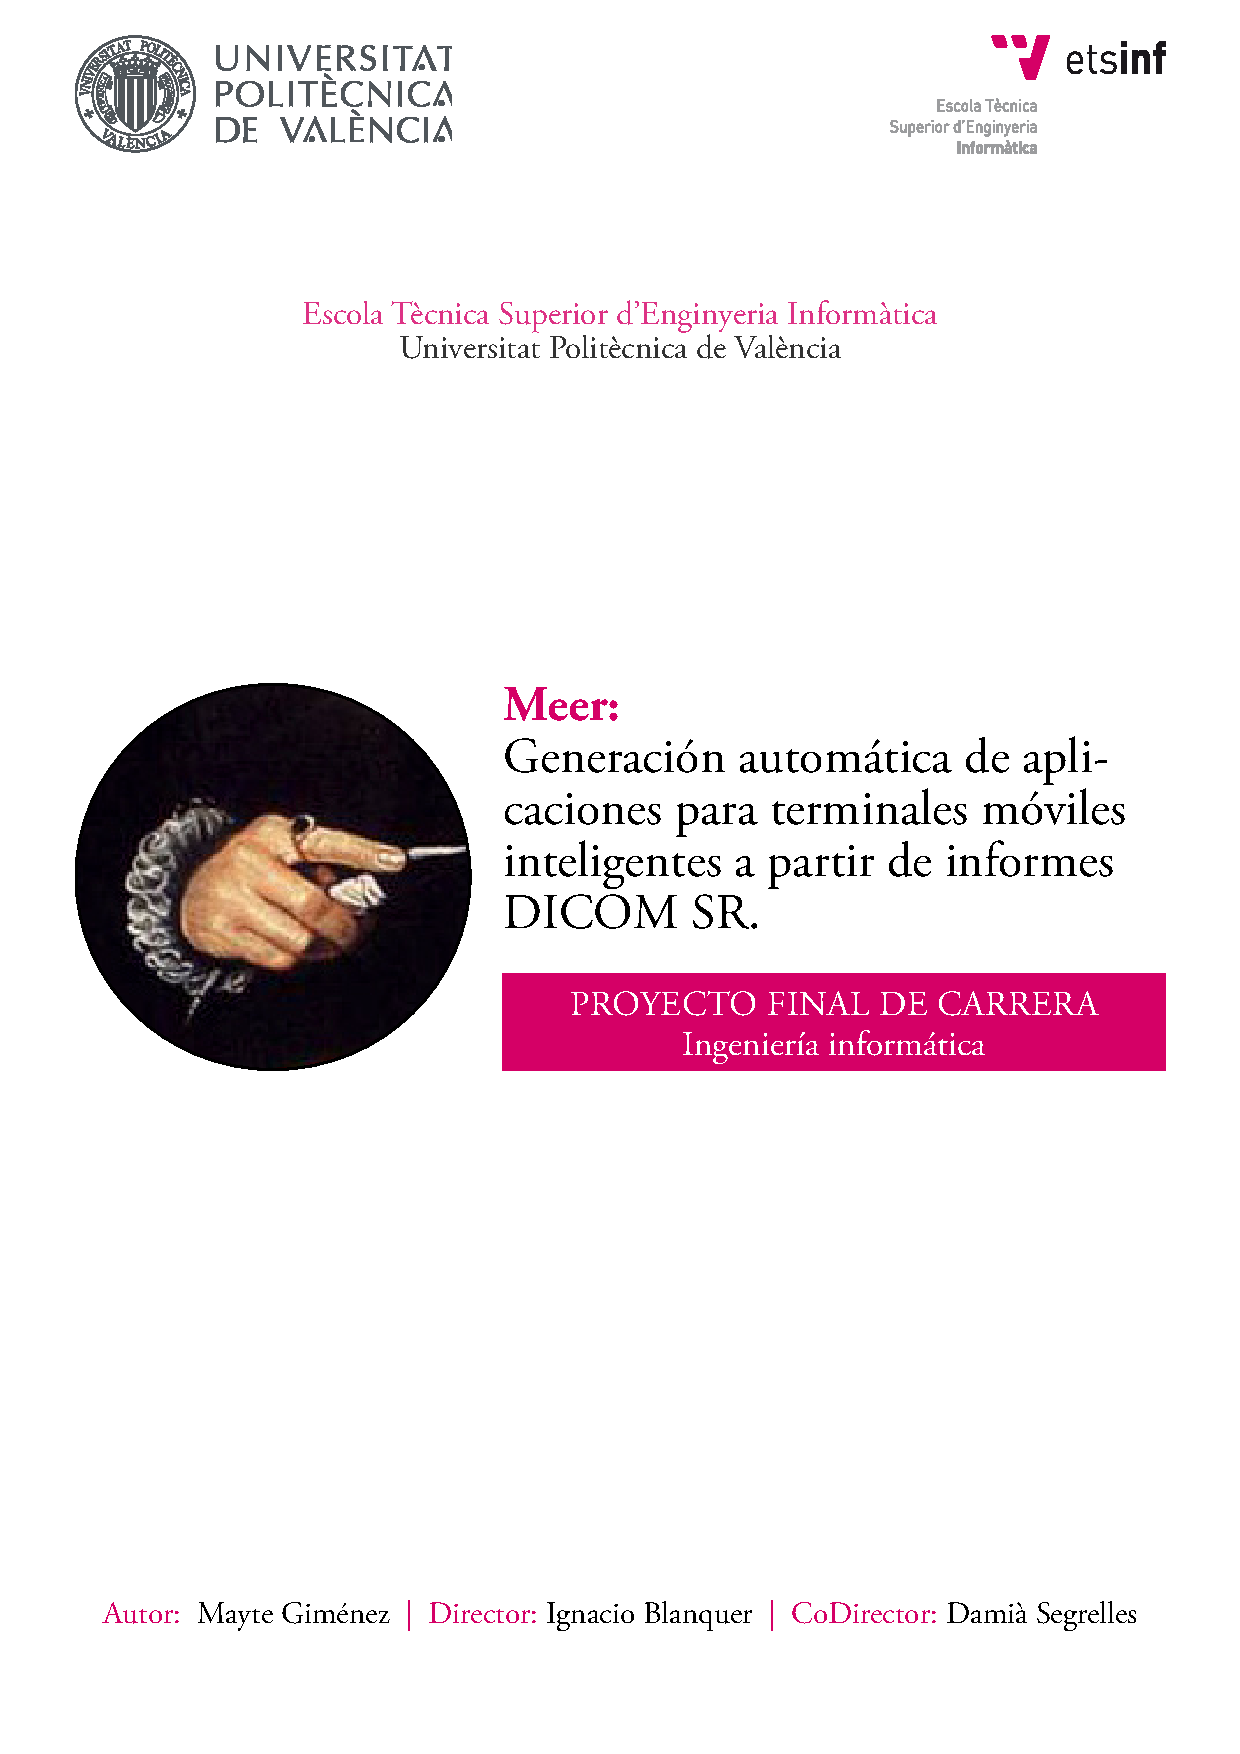
\includepdf[pages={1}]{./imgs/portada.pdf}

\begin{abstract}
El objetivo del siguiente Proyecto Fin de Carrera consiste en el desarrollo de una aplicación que a partir de un esquema de un informe médico, codificado en el estándar DICOM-SR, genere de manera automática una aplicación para dispositivos móviles de tipo Android de modo que facilite la adquisición de datos de pacientes e informes válidos.
\medskip  \par
El estándar Digital Imaging and Communication in Medicine (DICOM) define como tratar imágenes médicas desde su procesado hasta su comunicación. DICOM también especifica una extensión para soportar informes estructurados médicos (DICOM-SR), lo que ha permitido el desarrollo de distintas líneas de investigación basadas en este estándar. \medskip \par

En el ámbito médico, es fundamental que los datos adquiridos en los informes sean exhaustivos y fidedignos, sin embargo la gran versatilidad el estándar DICOM-SR hace que la propia adquisición de los datos sea un reto, en la que  la aparición y expansión de terminales móviles inteligentes pueden facilitar  la interacción entre el  usuario y la máquina. Estas tecnologías nos ofrecen la posibilidad de obtener datos de informes clínicos sin incrementar significativamente la carga de trabajo del personal médico. Por ello, son estas cualidades las que pretendemos explorar y explotar en este PFC, simplificando el proceso de adquisición de información para la obtención masiva de datos y de una mayor calidad.\par
Para ello se plantea como objetivo del PFC,  una aplicación para terminales Android, que permita al usuario introducir los datos de los informes estructurados basados en DICOMSR,  de un modo productivo, eficiente e intuitivo. La aplicación propuesta debe generar automáticamente a partir de un fichero plantilla donde se defina la estructura de informe DICOM-SR,  el código de la aplicación Android que proporcione la funcionalidad de inserción de informes.\par

\Keywords{DicomSR, Android, Python, Generación automática de código, imagen médica.}
\end{abstract}

\tableofcontents
\newpage

\listoffigures

\chapter{Introducción}
\section{Descripción del problema}\label{intro}
% Historia de los CADS y la imagen médica
Antes de profundizar en la descripción del problema que abordaremos en este proyecto final de carrera (PFC), hablaremos acerca del contexto en el que se inscribe.\medskip\par

La introducción de la imagen médica digitalizada ha transformado la práctica clínica. 
En la década de los 60 \cite{journals/cmig/Doi07} comienzan los esfuerzos por desarrollar líneas de investigación para el diagnóstico asistido por ordenador (CAD), pero no es hasta la década de los 80 cuando la tecnología permite que esta disciplina despegue. Solo como apunte para mostrar el impacto que tiene  el desarrollo de la imagen médica: la detección de cáncer de mama ha incrementado aproximadamente en un 10\% \cite{journals/cmig/Nishikawa07}, aunque podemos encontrar muchos otros ejemplos \cite{johnston1994effects, doi:10.1117/12.877968, kundel1975interpreting, Fujita:2008:CDE:1456710.1456735}.\medskip\par

% Historia de los PACs y DICOM
El formato de estas imágenes es crucial para el desarrollo de la investigación. Los Sistemas de Adquisición y Procesado de Imagen médica (PACs) \cite{huang2010pacs} contienen tanto el software como el hardware necesario para el tratamiento de la imagen médica.  Los principales elementos que forman los PACs son \cite{pianykh2012digital}:
\begin{itemize}
	\item \textit{Dispositivos de adquisición}: permiten la captura de la imagen médica. Estos dispositivos no tiene que compartir la misma tecnología de captura. Por lo que encontramos dispositivos de adquisición de imágenes como:
	\begin{itemize}
		\item Ultrasonidos.
		\item Resonancia magnética.
		\item Tomografía Axial Computarizada (TAC).
		\item Rayos X.
		\item \ldots
	\end{itemize}
	\item \textit{Archivos de la imagen médica}: servidores donde almacenar las imágenes.
	\item \textit{Estaciones de trabajo}: estaciones dónde los profesionales leen y trabajan con estas imágenes. 
\end{itemize}

 En la figura \ref{fig:pacs} vemos un esquema de los sistemas de adquisición y procesamiento de la imagen médica que acabamos de describir.\par
\begin{figure}[ht]
\centering
\includegraphics[scale=0.6]{./imgs/esquemas/pacs.pdf}
\caption{Componentes principales de los PACs}
\label{fig:pacs}
\end{figure}

\medskip\par

Y aunque en los inicios de estos sistemas cada fabricante comenzó desarrollando su propio formato para el majejo de las imagenes \cite{huang2011short, lemke2011short}, no tardaron en aflorar problemas derivados de la falta de un estándar para compartir y estudiar estas. Por este motivo surge en 1983 el estándar  Digital Imaging and Communication in Medicine (DICOM).\medskip\par

DICOM es un estándar \cite{bidgood1992introduction} desarrollado por el colegio Estadounidense de Radiología (ACR) y la asociación Nacional de Fabricantes eléctricos (NEMA), especifica no  solo el formato de las imágenes sino también como deben ser almacenadas, los protocolos para el intercambio de las mismas. \par
En los veinte años de vida el estándar no ha dejado de crecer. Se han desarrollado más de 160 suplementos al mismo que completan las carencias detectadas en su uso y se adaptan a las nuevas tecnologías. Entre el 2006 y el 2013, los temas en los que se ha centrado el foco de atención son la mejora en las tecnologías para la adquisición de las imágenes y los informes estructurados asociados a estas.\cite{dicomtrends}.
Precisamente de estos dos temas dan pie a dos líneas de investigación bien diferenciados en la literatura \cite{torres2012improving}:
\begin{itemize}
	\item \textit{Imagen médica}: cómo almacenar y procesar la información de las imágenes médicas. 
	\item \textit{Informes médicos}: informes estructurados con información de las imágenes.  
\end{itemize}
\medskip\par

Es precisamente en esta segunda rama de la investigación en la que nos centraremos en este PFC. Concretamente dentro del estándar DICOM, se especifica una extensión para tratar con los informes médicos estructurados, se trata del estándar DICOM-SR \cite{clunie2000dicom}, del cual relegamos una definición más en profundidad en el aparatado \ref{dicomSR}.\par
La correcta estructuración de los informes permite organizar el conocimiento sobre las imágenes, permitiendo comparar imágenes de manera precisa mediante métodos cuantificables, y con esta información mejorar el diagnóstico.  Estos informes estructurados, (así como la imagen médica) ofrece a los profesionales sanitarios herramientas de apoyo a la medicina basada en evidencias \cite{Sackett19973, Darlenski2010553, Elphick2004525}, y con los datos necesarios para entrenar a los sistemas de diagnostico asistidos por ordenador.\medskip\par

En la literatura podemos encontrar diferentes esfuerzos por mejorar el tratamiento del conocimiento contenido en los informes médicos\cite{BlanquerEspert:2009:COV:1528937.1529213,journals/jbi/TorresQEH12, journals/jamia/Tirado-RamosHL02}  y de la utilidad del uso de los informes DICOM-SR. \par
Pero lo que es evidente es que para que los estudios derivados de los informes médicos estructurados (DICOM-SR) sean eficaces necesitamos disponer de un conjunto amplio y preciso de estos. Aunque el uso de métodos estadísticos nos ayuda a paliar en  este problema, los modelos que se generen a partir de los datos y por extensión las conclusiones a las que pudiéramos llegar, serían en el mejor de los casos imprecisos. \par
Paradójicamente, nos encontramos con un cuello de botella en la adquisición de los datos en los informes DICOM-SR a partir de la imagen médica, ya que este proceso debe hacerlo un profesional. Rellenar formularios electrónicos pude ser una tarea tediosa, por lo que en la actualidad se emplea el reconocimiento del habla  para transcribir los informes de los profesionales como texto plano. Pero el lenguaje natural es impreciso por lo que se necesitan herramientas para aplicar la estructura de un informe DICOM a este texto plano \cite{sevenster2012aut, 9227155, citeulike:191295}. \medskip\par

Y es en este punto dónde encontramos el problema que queremos abordar. Necesitamos informes médicos estructurados, pero su adquisición es demasiado costosa y poco productiva de la manera tradicional, ya que la interacción requerida para que el usuario introduzca los datos es poco intuitiva y monótona, y las herramientas para aplicar la estructura del informe médico DICOM-SR al texto plano se ciñen a tipos de imagen concretos (Radiografías, radiologías,\ldots) debido a la complejidad de interpretar correctamente el lenguaje natural.\medskip\par

El otro elemento que nos hace falta para terminar de definir el problema, nos vincula con la solución que propondremos en el apartado \ref{solucion}, y es que afortunadamente las nuevas tecnologías nos ofrecen nuevas posibilidades. La interacción con los terminales móviles inteligentes han demostrado ser mucho más intuitiva y amigable para todo tipo de usuarios.\par
En los últimos años podemos encontrar trabajos que han comenzado a introducir terminales móviles inteligentes en el campo médico con resultados satisfactorios. \cite{journals/jdi/ChoudhriR11,20359897,journals/jdi/TangLLC04}\bigskip\par

Recapitulando, la existencia de estándares en la imagen médica ha facilitado el desarrollo de distintas líneas de investigación que han revolucionado la práctica clínica. \par
Los informes estructurados son una valiosa fuente de información médica, pero su adquisición requiere aumentar la carga de trabajo de los profesionales. \par
Los terminales móviles ofrecen nuevas formas de interactuar con los usuarios de manera más intuitiva, y su uso en el ámbito médico se ha probado productivo. \par


\section{Solución propuesta}\label{solucion}
La solución que se propone para el problema que hemos descrito en el apartado anterior, explota las ventajas que nos ofrecen los terminales móviles. Lo que se propone es desarrollar una aplicación que permita generar automáticamente una aplicación para terminales móviles inteligentes con el sistema operativo Android a partir de plantillas de los informes médicos estructurados (DICOM-SR).\medskip\par

Partimos de ficheros que sigan el estándar para informes médico DICOM-SR con la definición de la plantilla del tipo de informe en el que estamos interesados. Estos ficheros contienen información  acerca del tipo de informe, así como de todos los campos que deben estar presentes en el mismo; también contiene para cada campo información acerca del tipo, de las propiedades de cardinalidad, verificación de los mismos y posibles valores a asignar.\par

A partir de estos ficheros, extraeremos la información de los mismos y generamos el código necesario para crear un aplicación para terminales móviles inteligentes Android. Una vez hemos generado todos los ficheros necesarios (interfaz, modelo de clases, interacciones entre la interfaz de usuario, \ldots), los integraremos en el esqueleto de una aplicación Android estándar para este propósito, y de este modo tendremos el informe estructurado, convertido en una aplicación para terminales inteligentes.\par
En la figura \ref{fig:basic_schema}, podemos ver un esquema muy básico de la solución propuesta: la entrada del sistema es el fichero con la plantilla DICOM-SR, que se pasa a la aplicación en python que hemos desarrollado y esta genera una aplicación en Android con los datos del informe estructurado DICOM-SR. Entraremos en más detalles acerca de la arquitectura y la justificación de los detalles técnicos de la solución en los siguientes apartados.\bigskip\par

\begin{figure}[ht]
\centering
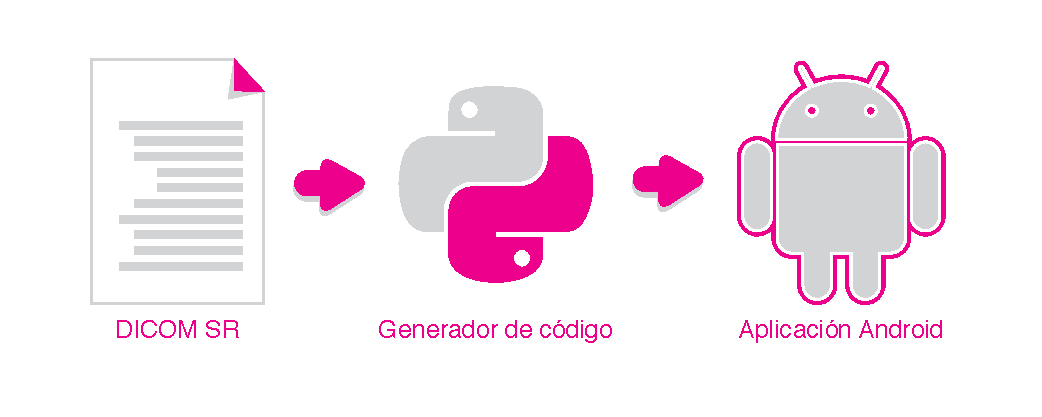
\includegraphics[scale=0.6]{./imgs/esquemas/simple.pdf}
\caption{Esquema básico}
\label{fig:basic_schema}
\end{figure}

El objetivo que pretendemos lograr con esta solución es claro: hacer uso de una interfaz de usuario muy intuitiva característica de los terminales móviles inteligentes, para interactuar con el usuario. Cuanto más podamos simplificar el trabajo del usuario a la hora de codificar los informes, más probablemente el profesional introduzca un número mayor de informes y de una forma más productiva. \medskip\par
La solución propuesta tiene varios puntos fuertes, que son los siguientes:
\begin{itemize}
\item Se trata de una solución \textit{genérica}. Independientemente del tipo de informe médico podemos de manera automática crear una aplicación Android que lo soporte.
\item Es \textit{adaptable} a los cambios en la plantilla DICOM-SR. Si añadimos nuevos campos, o modificamos el tipo de los mismos, la aplicación que se generaría cambiaría adaptándose a los cambios realizados en el informe.
\item Es \textit{configurarle}, ya el usuario podría decidir la configuración más intuitiva para él/ella.
\item La \textit{ubicuidad} de los terminales Android aporta al usuario la posibilidad al personal médico de comenzar la introcción de los datos en una pantalla táctil y continuar en una tableta. 
% TODO: Añadir la cita a los léxicos
\end{itemize}
\medskip\par

En definitiva, se trata de una solución que busca que los profesionales médicos introduzcan los datos de las imágenes que analicen en los informes médicos estructurados de tipo DICOM-SR  de una manera rápida e intuitiva. Los datos específicos de cada paciente introducidos por el profesional interactuando con la aplicación Android, se guardarán de nuevo en el formato estándar DICOM-SR. 

\chapter{Objetivos}

En este apartado enumeraremos los objetivos que se pretenden alcanzar por parte de la alumna durante el desarrollo de este proyecto final de carrera.\par
Esto nos permitirá acotar el alcance del proyecto y establecer los hitos a alcanzar, permitiendo elaborar una planificación lo más precisa posible.\medskip\par

Los objetivos a lograr son los siguientes:
\begin{itemize}
	\item Demostrar la habilidad para emprender un proyecto parcialmente autónomo a partir de lo estudiado durante el periodo de formación académica en la Ingeniería Informática.
	\item Comprender la estructura de los informes médicos de tipo DICOM-SR y ser capaz de interpretar su contenido.
	\item Desarrollar una aplicación que realice el análisis sintáctico y semántico de ficheros DICOM-SR.
	\item Desarrollar una aplicación Android genérica para generar interfaces que permitan la introducción de informes DICOM-SR en base a plantillas.
	\item Desarrollar una aplicación que a partir de un fichero DICOM-SR genere los ficheros necesarios para completar la aplicación Android básica para el informe concreto de entrada. 
	\begin{itemize}
		\item Comprender la generación de código haciendo uso de plantillas.
	\end{itemize}
	\item Realizar las pruebas pertinentes a la aplicación para un informe concreto. Estas pruebas las aplicaremos exhaustivamente a 4 ontologías:
	\begin{itemize}
		\item Exploración de mama.
		\item Mamografía.
		\item Ultrasonidos
		\item Resonancia magnética.
	\end{itemize}
	Y consistirán en realizar las siguientes tareas:
	\begin{itemize}
		\item Generar el código XML para soportar la internacionalización
		\item Generar el código XML que desarrolle la interfaz de usuario. 
		\item Generar el código XML con las propiedades de la aplicación Android.
		\item Generar el código java que codifique los modelos de clase del informe. 
		\item Generar el código java que codifique las interacciones entre actividades.
		\item Integrar todo el código generado dentro de la aplicación base de Android. 
		\item Comprobar su correcto funcionamiento en terminales físicos.
	\end{itemize}
\end{itemize}
\medskip\par
Aunque no sea estrictamente necesario, hemos creado un diagrama de Gantt que podemos ver en la figura \ref{fig:gantt}, que nos ayude a planificar el tiempo para lograr los objetivos que acabamos de describir.\par
\begin{figure}[ht]
\centering
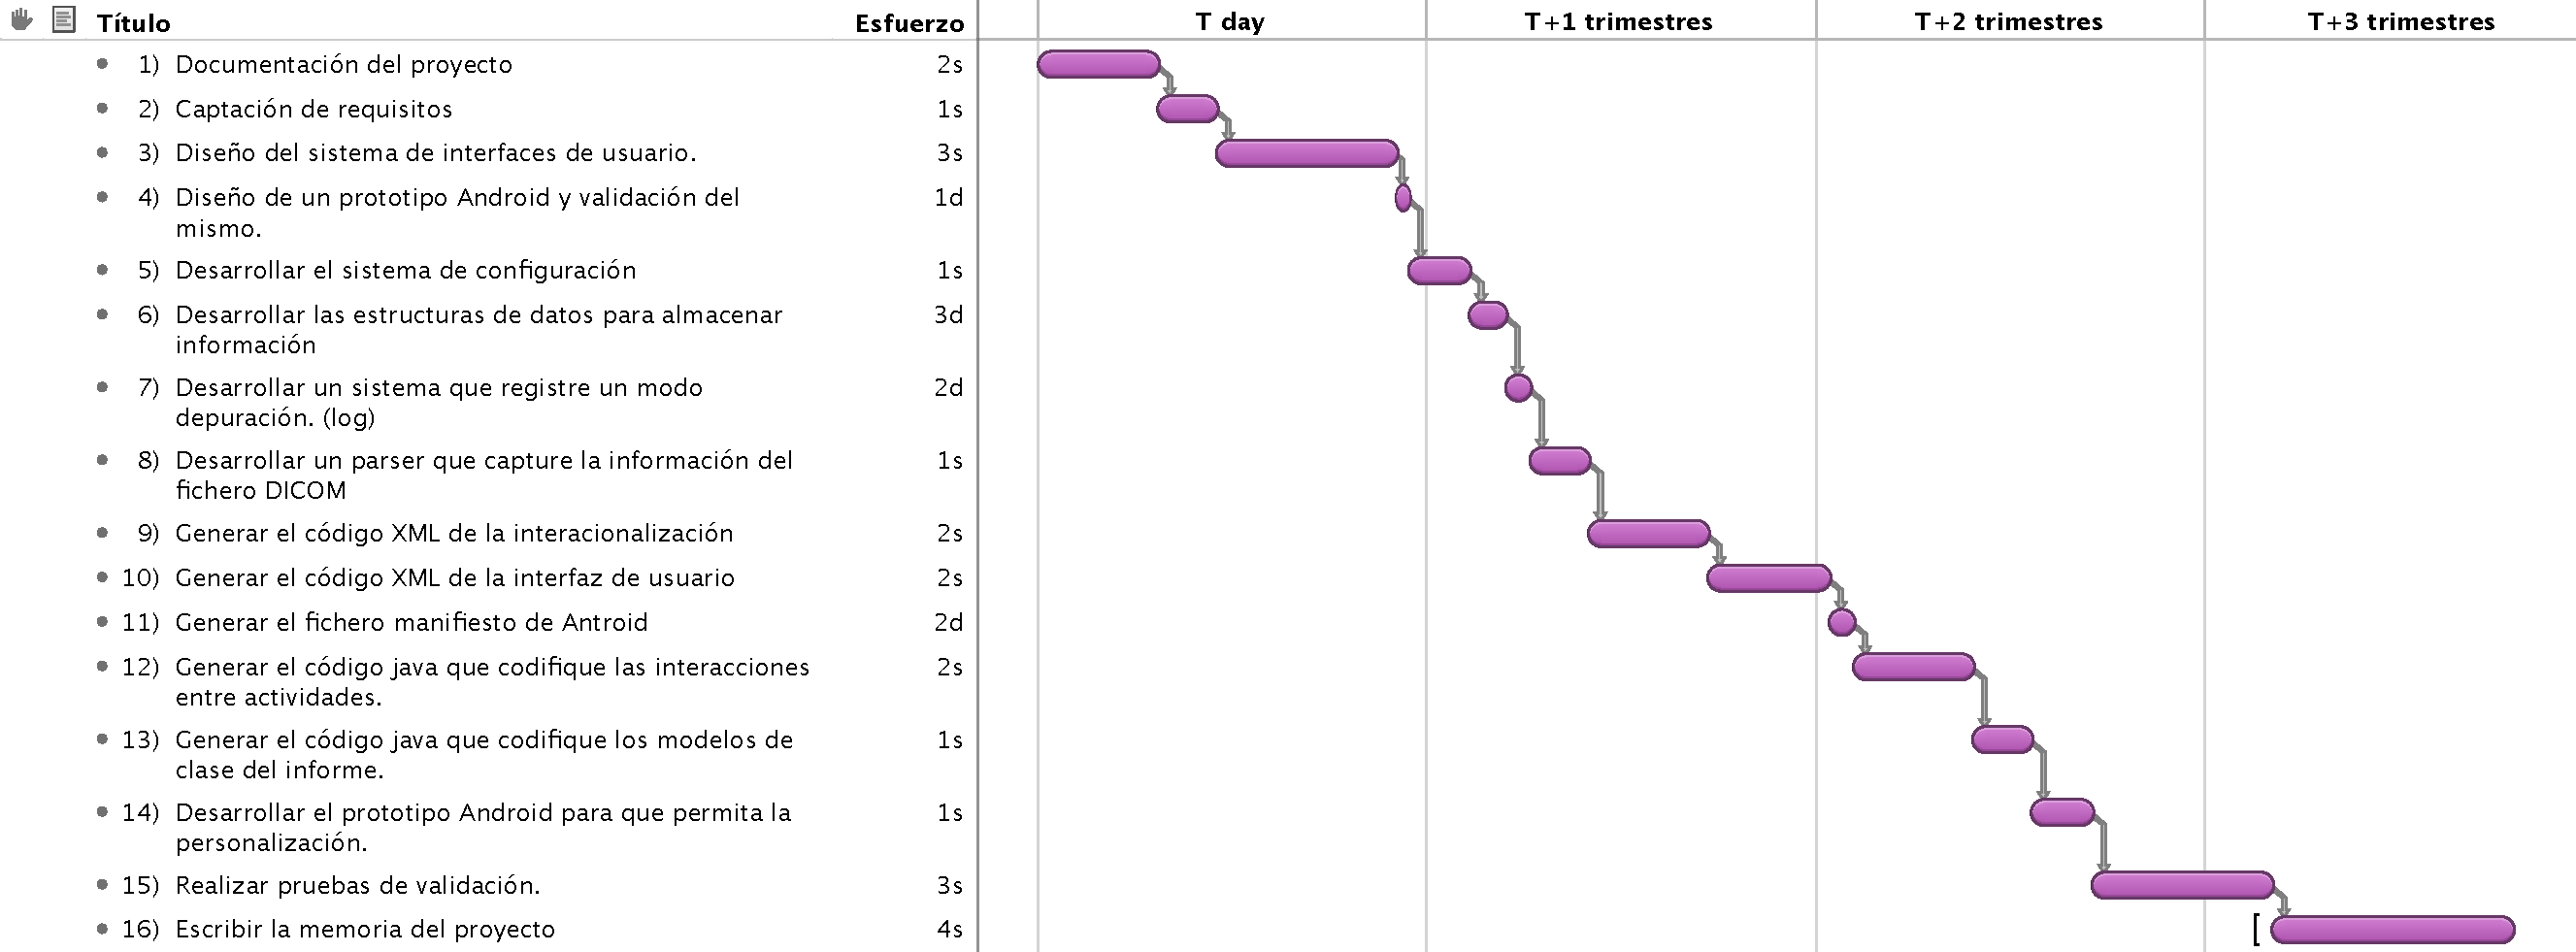
\includegraphics[scale=0.3]{./imgs/gantt.pdf}
\caption{Diagrama de Gantt}
\label{fig:gantt}
\end{figure}


\chapter{Estado del arte }\label{arte}
\chaptermark{Estado del arte}
Hasta este punto hemos introducido el problema y el contexto en el que ser circunscribe de manera generalista. En los siguientes apartados profundizaremos un poco más en el contexto del problema. Haremos un resumen del estado del arte de las áreas de conocimiento que vamos a trabajar. \medskip\par

\section{Imagen médica}
Situamos la primera imagen médica en 1895 con la imagen de rayos X de  Wilhelm Conrad Röntgen, pero no es hasta 1972 cuando encontraremos la primera imagen médica digitalizada: una tomografía computarizada de Godfrey Newbold Hounsfield. Paralelamente al desarrollo de la tecnología de los aparatos para la captación de imágenes hemos visto el desarrollo de las técnicas de la informática médica.\par
Encontramos en \cite{mantas2010recommendations}, una definición de lo que es la informática médica. Se trata del procesamientos sistemático de datos, información y conocimiento para la toma de decisiones óptima.\par
La medicina es un ámbito en que se puede aprovechar al máximo las nuevas posibilidades que nos ofrecen las tecnologías de la información. Es por esto que en los últimos 20 años hemos visto como ha florecido distintas líneas de investigación al rededor de la imagen médica.\par
Cuando hablamos de imagen médica nos referimos a un conjunto de técnicas y procesos para capturar imágenes del totales o parciales del cuerpo humano con propósitos cínicos.\cite{wiki:imgmedica}\par

En la literatura \cite{Muller20041,Maintz19981} podemos encontrar un repaso de los distintos dispositivos y tecnologías para captar imagen médica. Lo que es innegable es el gran impacto de la imagen médica en la práctica clínica. \medskip \par

Como afirmábamos en el apartado \ref{intro}, para hacer posible esta evolución son necesarios los estándares que permitan manipular las imágenes de manera óptima. Es precisamente por esto que se desarrolló el estándar de imagen médica DICOM. 
El acrónimo DICOM significa \textit{Imagen Digital y Comunicación en Medicina}. Por lo tanto no se trata únicamente del formato de la imagen sino que se diseñó para cubrir todas las necesidades vinculadas con la imagen médica. Necesidades como pueden ser: la compresión de imágenes, la comunicación, el almacenamiento, \ldots\par
Cada una de las necesidades específicas para el desarrollo de investigaciones y dispositivos relacionados con la imagen médica se recogen en el estándar y sus anexos que podemos encontrar en la web de la asociación Nacional de Fabricantes eléctricos (NEMA).\cite{nema}.\medskip\par

La literatura al respecto de la imagen médica en muy profusa. Por lo tanto, lo visto hasta el momento son únicamente los conceptos más básicos así como sus definiciones. La teoría sobre la imagen médica que hemos descrito forma parte de los cimientos sobre los que se sustenta este proyecto.\par

\section{Generación automática de código}\label{sec:generacion-codigo}
Otro de los pilares teóricos en los que se sustenta este proyecto es en la generación automática de código.\par
Cada una de las pruebas de imagen médica tiene asociado un informe DICOM-SR. Si nos planteáramos seguir un paradigma de programación diferente, necesitaríamos crear una aplicación Android para cada informe DICOM-SR. Aunque gran parte de este código fuera reutilizable, estaríamos desplazando el cuello de botella que ahora se encuentra en la captación de datos al desarrollo de aplicaciones.\par
Es por este motivo que optamos por la generación de código o traducción automática. Términos sinónimos en la literatura.\cite{802346}\medskip\par 
La generación automática de código es uno de los paradigmas de programación existentes y consiste en escribir programas que sean capaces de escribir el código fuente de otros programas basándose en modelos ontológicos.\par 
En nuestro caso los modelos ontológicos son las plantillas DICOM-SR. Para conseguir llevar a cabo esta tarea se dispone de un sistema de patrones que se instancian con los datos concretos, siguiendo unas reglas que son generalmente sencillas.\medskip\par
La generación automática de código es una de las líneas de investigación que más interés despierta en el ámbito de la ingeniería de software \cite{hinchey2005requirements}. Existe un buen número de razones para que esto sea así, a pesar de los desafíos que plantea este paradigma de programación. Entre los beneficios que ofrece la generación automática de código podemos enumerar los siguientes \cite{herrington2003code}:
\begin{itemize}
	\item \textit{Calidad}: El código generado mediante plantillas permite que la calidad sea consistente a lo largo de todo 	el software desarrollado y simplifica el proceso de aplicar parches que solucionen bugs. 
	\item \textit{Consistencia}: El estilo de programación mantiene una consistencia a lo largo de todo el software desarrolladoo.
	\item \textit{Más tiempo para el diseño del software y la arquitectura}: el análisis y desarrollo de la API en este paradigma es muy importante, por lo que se dedica más tiempo y recursos a captar los requisitos y crear la arquitectura. Estamos aprovechando el tiempo que de otro modo hubiéramos empleado en escribir manualmente el software.
	\item \textit{Abstracción}: la generación automática de código es independiente del lenguaje de programación, simplemente modificando el lenguaje de las plantillas podremos generar software en el lenguaje de programación que sea más conveniente. 
\end{itemize}
\medskip\par

La investigación actual tiene como gran reto el desarrollar modelos independientes del lenguaje y demostrar que el código que generan es computacionalmente equivalente al código generado por un desarrollador.\par
Sin embargo este enfoque queda fuera del alcance de nuestro proyecto. Lo que haremos es emplear las bases teóricas del paradigma de generación automática en nuestro desarrollo.\medskip\par
Existen diversas técnicas para generar código. Para este proyecto optamos por \textbf{generación parcial de clases}. La generación parcial de clases consiste en leer un fichero de texto con la información abstracta de las clases a generar, a continuación lee una serie de plantillas y con la información recogida de estas dos fuentes, generará el código necesario. Este código que hemos generado se integrará con el código escrito por ingenieros para formar la solución final.\par

En la figura \ref{fig:generacion} vemos como se aplica esta técnica de generación de código en nuestro ejemplo concreto. El sistema tendrá como entrada el informe médico de tipo DICOM-SR y una serie de plantillas, con esto generará el código necesario para que cuando lo integremos en la aplicación Android obtengamos una aplicación Android funcional específica para el informe de entrada. \par
\begin{figure}[ht]
\centering
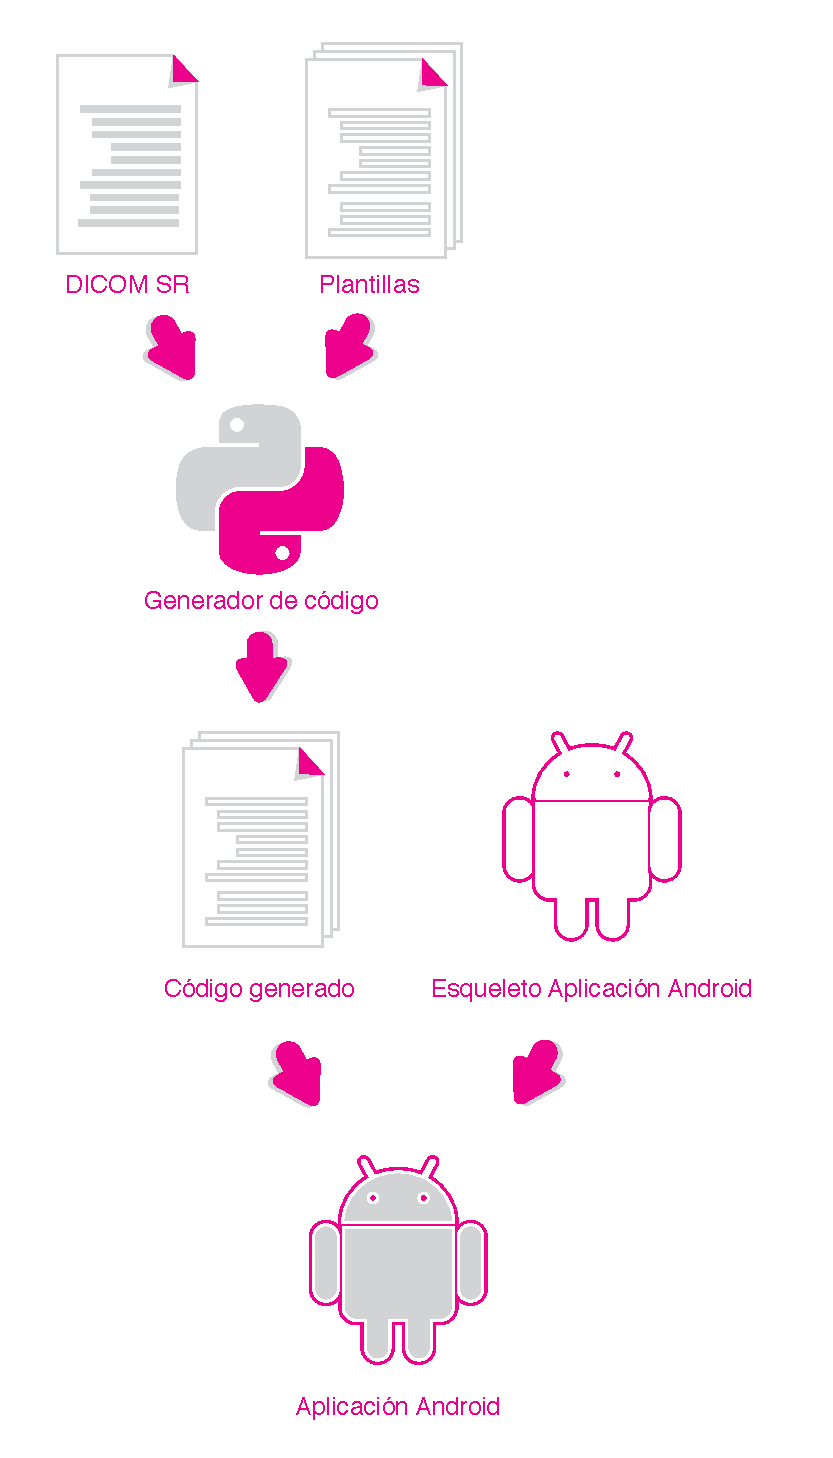
\includegraphics[scale=0.5]{./imgs/esquemas/generacion.pdf}
\caption{Generación parcial de clases}
\label{fig:generacion}
\end{figure}

\subsection{Desarrollo de software guiado por modelos}
El desarrollo de software guiado por modelos forma parte del paradigma de programación automática. De los paradigmas que descienden de la programación automática este es el que más se ajusta al trabajo que estamos presentando.\par
Consiste en desarrollar uno o varios modelos que representen el sistema y a partir de estos modelos se generará el software. Existen numerosas herramientas para definir modelos.\par
Según la literatura \cite{MDA} lo fundamental es que los modelos tengan las siguientes características:
\begin{itemize}
	\item Tan simples como sea posible (KISS).
	\item Canónico (DRY).
	\item Correcto nivel de abstracción.
	\item Separación de aspectos ( SoC ).
	\item Mantener modelos organizados y manejables.
	\item Independiente de la tecnología.
	\item Pragmáticos: sólo modelamos aquello que vayamos a emplear.
\end{itemize}
Podemos modelar todo o parte del sistema. Lo recomendable es que se modele aquello que varíe poco, con lo que el tiempo invertido en el modelado sea eficiente.\medskip \par

En nuestro caso el modelo viene determinado por el estándar soportado por los dispositivos PACs, es decir, utilizaremos los ficheros DICOM-SR como modelo para generar la aplicación.\par
Debido a las características del modelo, este proyecto no se adscribe dentro del desarrollo guiado por modelos tal y como se define en la literatura \cite{mdd}, pero si obviamos las características del modelo que vienen impuestas por los estándares médicos, seguimos la filosofía de este paradigma de programación, ya que a partir del modelo del sistema, el informe médico DICOM-SR, generamos el software con las características que el modelo define.\par


\section{Interacción persona-máquina y usabilidadad}\label{sec:UI}
\chaptermark{Usabilidad}
Por último, antes de cerrar este capítulo nos falta hablar del tercer pilar que sustenta este proyecto: la interacción persona-máquina.\par
Como hemos discutido en la introducción \ref{intro}, uno de los problemas a los que nos enfrentamos a la hora de recoger informes médicos es que rellenar estos informes es una tarea pesada para los profesionales clínicos que deben invertir mucho tiempo en la captación de requisitos. La tecnología per se no soluciona este problema, sino que nos da herramientas para afrontarlo. Lo que es importante es que realicemos un diseño de las interfaces de usuario centrándonos en las necesidades de las personas que utilizarán las aplicaciones.\medskip\par
El término Interacción Persona-Máquina (\textit{\textbf{H}uman-\textbf{C}omputer \textbf{I}nteraction} en inglés) no se popularizó hasta la década de los 80, aunque podemos encontrar raíces similares en los estudios de ergonomía de principios del siglo XX \cite{dix2004human}. Pero es con el auge de la informática y diseño de sistemas cuando el estudio de la Interacción persona-máquina comienza a desarrollarse plenamente de manera autónoma. Con la aparición de los ordenadores personales todo el mundo se convirtió en un usuario potencial y era necesario encontrar formas de interactuar adecuadamente con este nuevo público. \par
La Interacción Persona-Máquina se encarga del diseño, implementación y validación de las interfaces de usuario. Es decir, se encarga de modelar cómo los usuarios se relacionan con las máquinas.\medskip\par
Al desarrollar un proyecto de este tipo corremos el peligro cuando estemos absortos en los detalles técnicos de olvidar la importancia del diseño. Un buen diseño debe centrarse en las personas, y tiene un tremendo impacto en las tareas que realizan a pesar de que el diseño será transparente para los usuarios.\par
En ámbitos que incluyan sistemas críticos como puede ser la medicina, los fallos en el diseño de las interacciones pueden tener un gran coste económico y personal. A pesar de que nuestro ámbito de aplicación no es crítico tenemos presente que la aceptación del sistema por parte de los usuarios es un punto clave para resolver el problema que nos planteamos en este proyecto.\medskip \par
Los puntos claves para conseguir un buen diseño de interfaces se basan en que todo el sistema sea consistente y en solicitar información al usuario final acerca de sus impresiones y sensaciones con el diseño.\par 
Respecto a la consistencia, esta es una ventaja propia de la generación automática de código ya que mientras seamos consistentes en el diseño de las plantillas la aplicación final tendrá una aspecto coherente.\par
Para conseguir la información acerca de la idoneidad del diseño, el procedimiento consiste en crear un diseño y evaluar la satisfacción por parte de los usuarios, con las respuestas que obtenemos de nuestro usuarios, que idealmente será un grupo diverso que represente a las personas que utilizarán la aplicación, cambiamos el diseño y solicitamos de nuevo una evaluación del diseño. Idealmente seguiríamos iterando en el diseño de este prototipo hasta llegar a un punto en el los usuarios estén satisfechos con el resultado. En la práctica se llega a una solución de compromiso entre el tiempo empleado en el diseño y la satisfacción de los usuarios.\par
En nuestro proyecto hemos integrado los ciclos de diseño y validación de la interfaces dentro del desarrollo de la aplicación. En la fases iniciales de diseño, creamos las interfaces que se fueron refinando durante el proceso, y empleamos la aplicación Android que nos serviría de esqueleto dónde integrar el código generado como prototipo para poder validar el diseño.\medskip \par
Finalizamos este apartado recalcando la importancia del diseño, muchas veces denostado, en la aceptación por parte de los usuarios de las soluciones software que les proponemos. 



\chapter{Tecnologías empleadas en el proyecto}
En el capítulo \ref{intro} hemos planteado el problema y una posible solución al mismo. El objetivo tanto del capítulo anterior como este es el de sentar las bases teóricas y tecnológicas de la solución que hemos propuesto.\par 
Si en el capítulo  \ref{arte} repasábamos el estado del arte y sentábamos las bases teóricas del proyecto, en este capítulo describiremos la tecnología de la que hacemos uso para ejecutar de solución que proponemos. Además justificaremos los motivos que nos han llevado a seleccionar esta tecnología y no otra.\par

\section{DICOM-SR}\label{dicomSR}
En primer lugar hablaremos de la tecnología que nos impone el proyecto. Los PACs utilizan la extensión del estándar DICOM para informes estructurados(DICOM-SR) y como nuestro objetivo es que la solución se integre en el ecosistema existente en los centros médicos deberemos emplear este estándar.\medskip\par

\subsection{Definición}
DICOM-SR se incluye dentro del suplemento 23 del estándar de imagen médica DICOM. Describe una arquitectura de documento que permite compartir, almacenar y transmitir información de informes médicos estructurados \cite{hussein2004dicom}.\par
Se diseñó con la intención de suplir la brecha entre la información contenida en las imágenes y la información que los profesionales médicos introducen en estos. Los ficheros DICOM-SR almacenan de forma no ambigua y jerárquica todos los conceptos que podemos encontrar en un informe médico tradicional y además pueden incluir referencias a:
\begin{itemize}
	\item Imágenes en formato DICOM. 
	\item Informes de estudios previos.
	\item Detalles de las imágenes.
\end{itemize}\par\medskip\par
El estándar define el modelo de la información y cómo debe gestionarse el documento, lo que permite personalizar muchos aspectos de la implementación final\cite{hussein2004dicom2}.\par
Sin embargo al tratarse de un estándar bastante complejo, han surgido soluciones bastante dispares, entre las que podemos encontrar:
\begin{itemize}
	\item Una implementación basada en la orientación objetos integrando el estándar DICOM-SR en la estructura de XML.\cite{tirado2002information}
	\item Una implementación extendiendo el modelo de objetos de documento XML (DOM).\cite{doi:10.1117}
	\item Una implementación en C y C++ del estándar. \cite{Riesmeier2001795}
\end{itemize}
\par
Desde la Asociación Nacional de Fabricantes eléctricos (NEMA), se están haciendo esfuerzos por unificar los criterios y seguir avanzando en la definición del estándar.\par
Para este proyecto se emplea una implementación en la que el informe se estructura en un XML. Expondremos los detalles de los ficheros DICOM-SR con los que trabajaremos en los apartados \ref{dicomsr:ficheros},\ref{dicomsr:plantillas}, \ref{dicomsr:vocabulario} y \ref{dicomsr:internacionalizacion}.\par

\subsection{Beneficios del estándar DICOM-SR}\label{dicom:beneficios}
A pesar de los problemas que surgen en la definición y en la implementación del estándar, los beneficios que aporta su desarrollo merecen el esfuerzo. Podemos encontrar un resumen exhaustivo de las ventajas de DICOM-SR en el siguiente artículo \cite{noumeir2006benefits}. Entre las mejoras que aporta a la práctica clínica más relevantes encontramos: 
\begin{itemize}
	\item Mejora la comunicación entre los profesionales, al utilizar un léxico estándar no hay lugar a traducciones o 	interpretaciones erróneas. 
	\item Los informes son más precisos y concisos. Los profesionales rellenan el informe utilizando los códigos adecuados sin 	las estructuras gramaticales que serían necesarias al redactar los informes de modo tradicional. 
	\item Se evitan los errores gramaticales y de transcripción.
	\item La interpretación de los informes es más sencilla y permite una interpretación asistida por ordenador. 
	\item Las imágenes DICOM y los informes DICOM-SR comparten la misma cabecera que contiene información acerca del paciente, 	lo que mejora el registro de información médica.
	\item El informe incluye medidas numéricas de las evidencias encontradas, que redundará en la precisión del informe.
	\item Permite ejecutar acciones automáticas sobre los informes permitiendo la minería de datos.
	\item Se enfatizan los contenidos. El informe en DICOM-SR no guarda información de cómo debe mostrarse al usuario, separa el contenido de la presentación de los datos.
	\item Permite la transformación a otros formatos. 
	\item Permite la integración con sistemas que reconozcan el habla. 
\end{itemize} 
Como podemos comprobar el desarrollo del estándar tiene un impacto beneficioso directamente sobre la práctica clínica, es por esto que en los últimos 5 años ha crecido el interés de la comunidad científica por explotar el estándar DICOM-SR.\par

\subsection{Estructura de un informe médico estructurado} \label{dicomsr:ficheros}
A continuación describiremos las características de un informe médico DICOM-SR representado siguiendo el formato XML.\par
En un fichero XML que contiene un informe médico DICOM-SR, la información se organiza mediante contenedores \textit{<CONTAINER>}. Los contenedores no almacenan la información, únicamente la estructuran. Los contenedores tienen hijos \textit{<CHILDS>}, y es dentro de los hijos dónde se almacena la información correspondiente a un informe concreto. Cada elemento de información se agrupa con las etiquetas con el tipo del valor que designan el tipo de elemento que se almacena en el campo. En nuestro PFC soportamos las siguientes, aunque existen otros muchos:
\begin{itemize} 
 	\item \textit{<DATE>}: almacena fechas.
 	\item \textit{<TEXT>}: almacena texto sin formato.
 	\item \textit{<NUM>}: almacena enteros o boleanos.
 	\item \textit{<CODE>}: almacena campos multievaluados.
 \end{itemize}
Dentro de las secciones definidas por estas etiquetas de tipo valor encontramos los datos del informe médico en pares de elementos clave-valor. Para designar la clave utilizamos la etiqueta \textit{<CONCEPT\_NAME>}, mientras que para referirnos al valor de este contenedor utilizamos la etiqueta \textit{<VALUE>}.
En el ejemplo de la figura \ref{dicom-report-tags} podemos ver como se codifica el identificador \textit{M001} de una lesión de tipo masa. Vemos un contenedor que abarca el concepto \textit{masa} y entre los hijos encontramos el identificador de la masa que es de tipo texto.\par
En el campo valor, \textit{<VALUE>}, podremos encontrar entre otros:
\begin{itemize}
	\item Texto plano.
	\item Valores numéricos con sus unidades.
	\item Fechas.
	\item Referencias a imágenes DICOM.
	\item \ldots
\end{itemize}\par

Un punto importante para alcanzar los objetivos descritos en \ref{dicom:beneficios}, es trabajar con un léxico limitado y bien conocido, por lo que se utilizan diccionarios de conceptos médicos para identificar cada concepto de los que puede aparecer en un informe.Cada concepto del informe se identifica por su \textit{CONCEPT\_NAME} que está formado por tres elementos:
\begin{itemize}
	\item \textit{CODE\_SCHEMA}: identifica el diccionario dónde se encuentra el término que estamos definiendo.
	\item \textit{CODE\_VALUE}: es el código al término médico definido.
	\item \textit{CODE\_MEANING}: contiene una descripción en texto plano del término para que sea legible por el usuario.
\end{itemize}
La combinación de \textit{CODE\_SCHEMA} y \textit{CODE\_VALUE} identifica de modo único un concepto dentro del informe.\par
De nuevo empleando el ejemplo \ref{dicom-report-tags}, vemos que el concepto \textit{masa} se encuentra en el diccionario \textit{RADLEX} con el código \textit{RID3874}.\medskip\par

\lstset{escapechar=@,style=dicom}
\renewcommand*\lstlistingname{Código}
\begin{lstlisting}[label=dicom-report-tags,caption=Fragmento de un informe estructurado de una exploración de mama]
		  ...
          <CONTAINER>
            <CONCEPT_NAME>
              <CODE_VALUE>RID3874</CODE_VALUE>
              <CODE_SCHEMA>RADLEX</CODE_SCHEMA>
              <CODE_MEANING>Mass</CODE_MEANING>
            </CONCEPT_NAME>
            <CHILDS>
              <TEXT>
                <CONCEPT_NAME>
                  <CODE_VALUE>118522005</CODE_VALUE>
                  <CODE_SCHEMA>SNOMED-CT</CODE_SCHEMA>
                  <CODE_MEANING>Identifier</CODE_MEANING>
                </CONCEPT_NAME>
                <VALUE> M001 </VALUE>
              </TEXT>
              ...
\end{lstlisting}

La información DICOM-SR del informe rellena el árbol XML. Existen implementaciones del estándar que hacen uso de etiquetas específicas para indicar las relaciones entre los contenedores DICOM, pero debido a que los ficheros XML almacenan la información per se en forma de árbol estas etiquetas son redundantes.\par
En la figura \ref{fig:dicom-report} se puede ver un esquema del árbol de conceptos de un informe siguiendo el formato DICOM-SR. Se trata de un exploración de mama, en la que se ha encontrado una masa en la mama derecha y dos asimetrías en la mama izquierda. Los campos de tipo valor, es decir los atributos del contenedor padre los representamos utilizando los cuadrados grises. Mientras que los contenedores, que no almacenan información pero estructuran el informe, los representamos con los cuadrados magentas.\par
Podemos encontrar el fichero DICOM-SR completo del informe que representa esta figura en el apéndice \ref{dicom-sr}.	\par

\begin{figure}[ht]
\centering
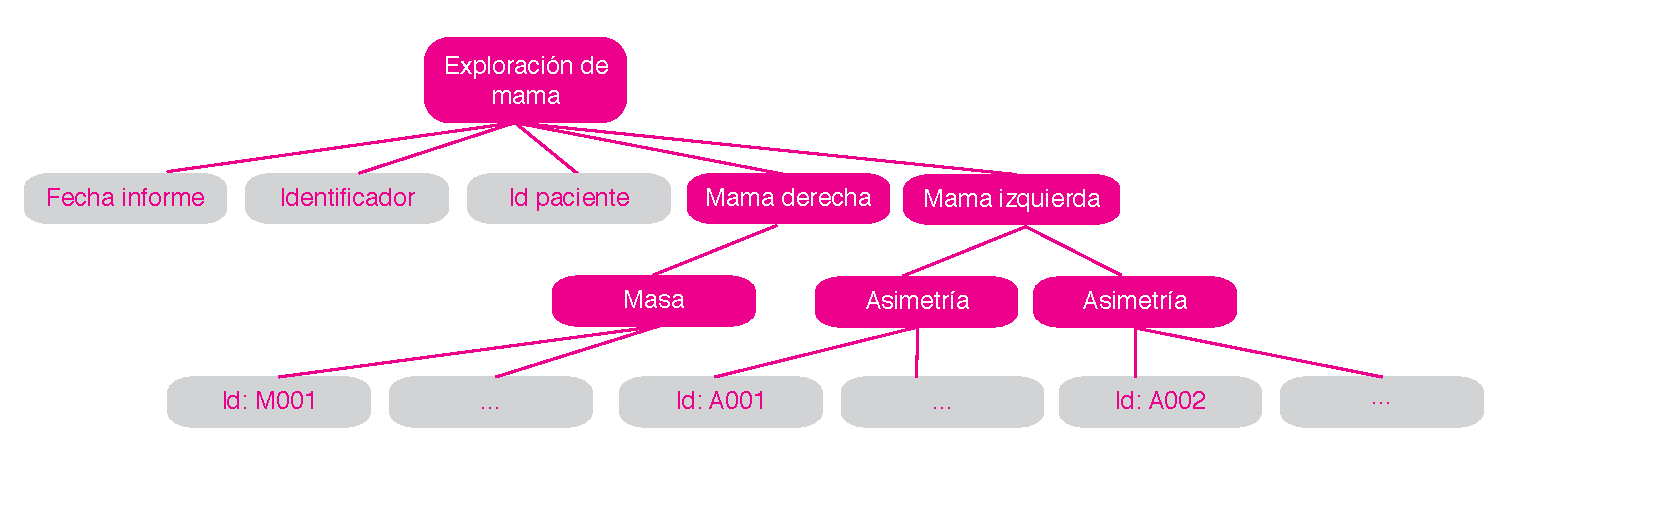
\includegraphics[scale=0.7]{./imgs/esquemas/dicomsrTreeReportA.pdf}
\caption{Representación del árbol XML de un informe en formato DICOM-SR}
\label{fig:dicom-report}
\end{figure}

\subsection{Estructura de una plantilla para un informe médico estructurado}\label{dicomsr:plantillas}
El estándar DICOM-SR, permite gran flexibilidad a la hora de escribir los informes estructurados. Esta característica puede complicarnos mucho el trabajo si cada especialista médico escribiera los informes siguiendo criterios correctos según el estándar pero aleatorios.
Para solucionar esto se crean las plantillas.
Las plantillas describen cómo debe ser un informe de tipo DICOM-SR, incluye los conceptos que debe tener así como las relaciones de jerarquía entre ellos y las propiedades que deben cumplir: si los conceptos son obligatorios o no, si pueden repetirse a lo largo del informe, \ldots\par 
Únicamente se guardan los conceptos en las plantillas, los campos correspondientes a los valores  \textit{<VALUE>} se incluirán después cuando el profesional rellene los datos para un paciente concreto.\par
El formato de las plantillas DICOM-SR es muy similar al de los informes DICOM. Carecen de las etiquetas \textit{<VALUE>} pero incluyen etiquetas \emph{<PROPERTIES>} para especificar las propiedades que deben tener los campos.\par
En el ejemplo de código \ref{dicom-template-mass} vemos como se almacenaría un concepto de tipo masa en una plantilla para la exploración de mama. Este contenedor podrá aparecer 0 o más veces en el informe final  (\textit{<CARDINALITY max=``-1'' min=``0''/>}) y lo introduce el usuario (\textit{<CONDITION\_TYPE type=``U''/>}).\medskip\par


\lstset{escapechar=@,style=dicom}
\renewcommand*\lstlistingname{Código}
\begin{lstlisting}[label=dicom-template-mass,caption=Fragmento de un plantilla informe estructurado: codificar una anomalía de tipo masa en una exploración de mama.]
		  ...
            <CONCEPT_NAME>
              <CODE_VALUE>RID3874</CODE_VALUE>
              <CODE_SCHEMA>RADLEX</CODE_SCHEMA>
              <CODE_MEANING>Mass</CODE_MEANING>
            </CONCEPT_NAME>
            <PROPERTIES>
              <CARDINALITY max="-1" min="0"/>
              <CONDITION_TYPE type="U"/>
              <EXPRESION_CONDITION xquery=""/>
            </PROPERTIES>
          ...
\end{lstlisting}

Además, en las plantillas de los contenedores se pueden incluir etiquetas para indicar la unidad de medida de los mismos, dentro de las etiquetas \emph{<UNIT\_MEASUREMENT>}. Estas etiquetas también servirán como modificadores como es el caso del ejemplo \ref{dicom-template-bool}, donde la etiqueta para el tipo del valor número, \textit{<NUM>}, se modifica de modo que el valor que introduzca el usuario será de tipo boleano, es decir sólo se permiten los valores 0 y 1. Así el concepto ``Cuadrante superior exterior de la mama derecha'' tendrá el valor verdadero o falso si la anomalía se sitúa en esa posición de la mama.\medskip\par

\lstset{escapechar=@,style=dicom}
\renewcommand*\lstlistingname{Código}
\begin{lstlisting}[label=dicom-template-bool,caption=Fragmento de una plantilla de un informe estructurado: codificar un atributo de tipo booleano.]
		  ...
              <NUM>
                <CONCEPT_NAME>
                  <CODE_VALUE>RID29929</CODE_VALUE>
                  <CODE_SCHEMA>RADLEX</CODE_SCHEMA>
                  <CODE_MEANING>Upper Outer Quadrant of Right Female Breast</CODE_MEANING>
                </CONCEPT_NAME>
                <PROPERTIES>
                  <CARDINALITY max="1" min="1"/>
                  <CONDITION_TYPE type="M"/>
                  <EXPRESION_CONDITION xquery=""/>
                  <DEFAULT_VALUE value="0"/>
                  <UNIT_MEASUREMENT>
                    <CONCEPT_NAME>
                      <CODE_VALUE>000000001</CODE_VALUE>
                      <CODE_SCHEMA>UNIT_MEASUREMENT</CODE_SCHEMA>
                      <CODE_MEANING>Boolean Units</CODE_MEANING>
                    </CONCEPT_NAME>
                  </UNIT_MEASUREMENT>
                </PROPERTIES>
              </NUM>
              ...
\end{lstlisting}

Las plantillas deben sintetizar el conocimiento de los especialistas técnicos que conozcan el estándar DICOM-SR y los profesionales médicos que conocen las características que deben tener los informes de las pruebas clínicas, por lo que será imprescindible la colaboración entre los profesionales de ambos ámbitos para crear las plantillas DICOM-SR.\medskip\par

Utilizamos estas plantillas como entrada para nuestro sistema. Tenemos una plantilla por ontología de exploración médica. Para este proyecto estamos trabajando con 4 ontologías diferentes.
\begin{itemize}
	\item Exploración de mama.
	\item Mamografía.
	\item Escáner de ultrasonidos.
	\item Resonancia Magnética
\end{itemize}

En el caso de las plantillas la información también se estructura en forma de árbol. En el apéndice \ref{dicom-sr-template}, hemos incluido una plantilla truncada para el informe de una exploración de mama. En este apéndice se describe una plantilla que permite introducir lesiones de tipo masa en la mama derecha y asimetrías en la mama izquierda. El esquema \ref{fig:dicom-template} muestra esta plantilla con su  forma arbórea.\medskip\par

\begin{figure}[ht]
\centering
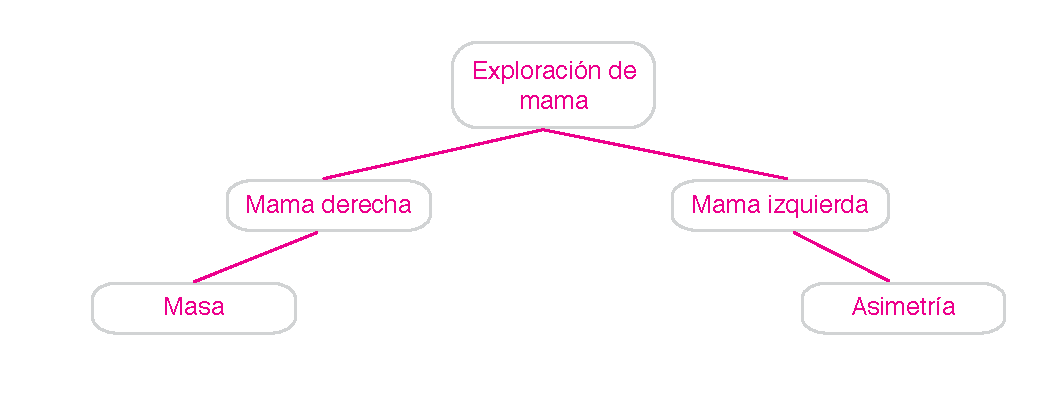
\includegraphics[scale=0.7]{./imgs/esquemas/dicomTreeTemplate.pdf}
\caption{Representación del árbol XML de una plantilla para un informe en formato DICOM-SR}
\label{fig:dicom-template}
\end{figure}


\subsection{Vocabulario}\label{dicomsr:vocabulario}
Un punto en el que hemos hecho hincapié es en la ventaja que supone que los informes hagan uso de un vocabulario estandarizado. Esto permite hacer referencia a conceptos concretos de manera precisa. Evitando los problemas que supone la barrera lingüística y la falta precisión del lenguaje natural.\medskip\par
También en lo que respecta al uso de vocabularios médicos DICOM-SR permite gran flexibilidad, permitiendo a los usuarios seleccionar el léxico que más les convenga en cada momento. En un mismo informe estructurado DICOM-SR pueden aparecer varios vocabularios.\par
Los vocabularios más habituales que podemos encontrar son: 
\begin{itemize}
	\item \emph{RadLex}: léxico desarrollado para cubrir las necesidades de la imagen radiológica. Contiene más de 30.000 términos \cite{langlotz2006radlex}.
	\item \emph{ICD-10}: léxico generalista que contiene un índice internacional de enfermedades y problemas relacionados con la salud. Está traducido en 42 idiomas \cite{world2004icd}.
	\item \emph{SNOMED-CT}: se considera la terminología clínica que más términos abarca y que soporta más lenguajes \cite{stearns2001snomed}. Se está convirtiendo en un estándar de facto al estar apoyado por numerosos gobiernos internacionales \cite{snomed-gov}.
\end{itemize}
\medskip\par
Sin embargo estos léxicos también presentan algunos inconvenientes: los conceptos pueden aparecer en varios léxicos, existen léxicos muy específicos para un país o idioma\ldots\medskip\par
Para este proyecto utilizaremos los siguientes léxicos:
\begin{itemize}
 \item Estándares internacionales:
 \begin{itemize} 
  \item \emph{RadLex}. 
  \item \emph{SNOMED-CT}.
 \end{itemize}
 \item Vocabularios definidos por nostros:
 \begin{itemize} 
  \item \emph{TRENCADIS\_MAMO}.
  \item \emph{UNIT\_MEASUREMENT}.
 \end{itemize}
 \end{itemize}
  \par
	
\subsection{Internacionalización}\label{dicomsr:internacionalizacion}
Las máquinas pueden trabajar con códigos como los que se almacenan en los léxicos médicos, incluso para algunas tareas puede ser incluso más beneficioso que tener que lidiar con secuencias de caracteres, especialmente si estos incluyen caracteres especiales. Pero las personas necesitamos el vocabulario para comprender los conceptos y poder trabajar con ellos.\medskip \par

La internacionalización y localización consiste precisamente en adaptar el software a los distintos idiomas y a las diferencias regionales como puedan ser los formatos de las divisas. No se trata únicamente de traducir las cadenas de texto.\par 
La internacionalización es la primera parte del proceso, consiste en diseñar y preparar el software que vamos a desarrollar y la localización es el proceso de adaptar el software creado a los distintos idiomas que se soporten \cite{Uren:1993:ISI:562752}. \medskip\par

Para presentar el informe a los profesionales médicos hacemos uso del texto codificado en las etiquetas \emph{<CODE\_MEANING>}. Sabiendo que algunos de los léxicos que se pueden incluir dentro un informe estructurado DICOM-SR están traducidos a múltiples idiomas, necesitamos encontrar una manera de que el significado del concepto sea diferente para cada lenguaje.\par
El estándar DICOM-SR especifica que las cadenas que se introduzcan en el campo \emph{<CODE\_MEANING>} pertenezcan al léxico con el que se esté trabajando, lo que no implica que estos textos deban estar en inglés, pero restringe la posibilidad de implementar soluciones en las que las traducciones no provengan de fuentes oficiales, porque esto nos conduciría de nuevo a la confusión semántica que pretendíamos evitar con el uso de vocabularios.\par
La solución que se propone en la literatura \cite{clunie2000dicom}, es hacer uso de la codificación del fichero para deducir el lenguaje del mismo, pero aunque se trata de una solución sencilla que no implica tener que trasmitir ni almacenar más información, si varios idiomas pueden utilizar la misma codificación no hay ninguna manera de diferenciarlos siguiendo este método. La otra solución que se propone es utilizar una etiqueta para identificar el idioma. Los ficheros XML con los que trabajamos optan por la segunda opción. Utilizan la etiqueta \emph{<CODE\_MEANING>} para un primer idioma y \emph{<CODE\_MEANING2>} para un segundo como podemos ver en el ejemplo \ref{code-meaning}.\par

\lstset{escapechar=@,style=dicom}
\renewcommand*\lstlistingname{Código}
\begin{lstlisting}[label=code-meaning,caption=Internacionación y localización en ficheros DICOM-SR.]
		  ...
  <CONTAINER>
    <CONCEPT_NAME>
      <CODE_VALUE>RID10312</CODE_VALUE>
      <CODE_SCHEMA>RADLEX</CODE_SCHEMA>
      <CODE_MEANING>Resonancia Magnética</CODE_MEANING>
      <CODE_MEANING2>Magnetic Resonance Imaging</CODE_MEANING2>
    </CONCEPT_NAME>
              ...
\end{lstlisting}


En nuestro PFC trabajaremos con plantillas localizadas para castellano e inglés como las que hemos visto en el ejemplo \ref{code-meaning}, así como con plantillas únicamente en inglés sin localizar como los fragmentos vistos en los ejemplos \ref{dicom-report-tags}, \ref{dicom-template-mass} y \ref{dicom-template-bool}

\section{Android}
Los teléfonos móviles inteligentes y las tabletas son tecnologías que ya llevan bastante tiempo entre nosotros, pero es en los últimos cinco años cuando la tecnología ha crecido exponencialmente. El índice de penetración en el mercado supera el 50\% en el caso de China y Estados Unidos, mientras que en Europa encontramos porcentajes inferiores, alrededor del 25\% pero las previsiones estiman que estas tasas crezcan rápidamente \cite{wiki:smartphones}.\par
La integración de dispositivos, la posibilidad de acceder a Internet y sobretodo la simplicidad de su uso fomentada por la posibilidad de interactuar con el dispositivo a través de la pantalla táctil, mucho más intuitivo que el teclado y el ratón, junto con un muy buen diseño de interfaces han facilitado la gran adopción de esta tecnología ya que han conseguido ampliar el espectro de usuarios potenciales\medskip\par

Un punto fundamental en el éxito de estas tecnologías es sin duda el nacimiento de Android.\par
Android es un sistema operativo basado en Linux, diseñado para trabajar con dispositivos móviles con pantallas táctiles. Fue desarrollado inicialmente por Android Inc., que fue comprada por Google en 2005. En el 2007 se forma la Open Handset Alliance: un conglomerado de empresas de hardware, software y telecomunicaciones cuyo objetivo es el de crear un entorno estandarizado para el desarrollo de dispositivos móviles. La OHA disponía de todos los agentes necesarios para revolucionar el mercado de las comunicaciones móviles y es en Octubre de 2008 cuando aparece el primer teléfono inteligente el HTC Dream que corría un Android 1.0. \cite{wiki:android}.\medskip\par

A partir de este momento el desarrollo de Android no ha dejado de crecer, convirtiéndose en una tecnología clave.\par
Como ya se ha comentado en el apartado \ref{intro}, el uso de terminales móviles inteligentes en la práctica clínica para trabajar con imagen médica ha dado resultados muy satisfactorios. Por lo tanto, es obvio pensar que una aplicación para recopilar informes médicos sobre Android tendrá mejor acogida por parte del personal médico, ya que es más sencillo e intuitivo introducir los datos de los informes DICOM-SR. Y al facilitar esta tarea al personal médico, es más factible que podamos adquirir más informes DICOM-SR con los que realizar estudios posteriores.\par 

\subsection{Arquitectura}
En este apartado hablaremos brevemente de la arquitectura de Android.\par
Android es un sistema operativo abierto basado en Linux, cuyo núcleo está escrito en C y C++, y que fundamentalmente tiene soporte para Java. Google libera periódicamente el código del sistema operativo bajo la licencia Apache.\par 
\begin{figure}[ht]
\centering
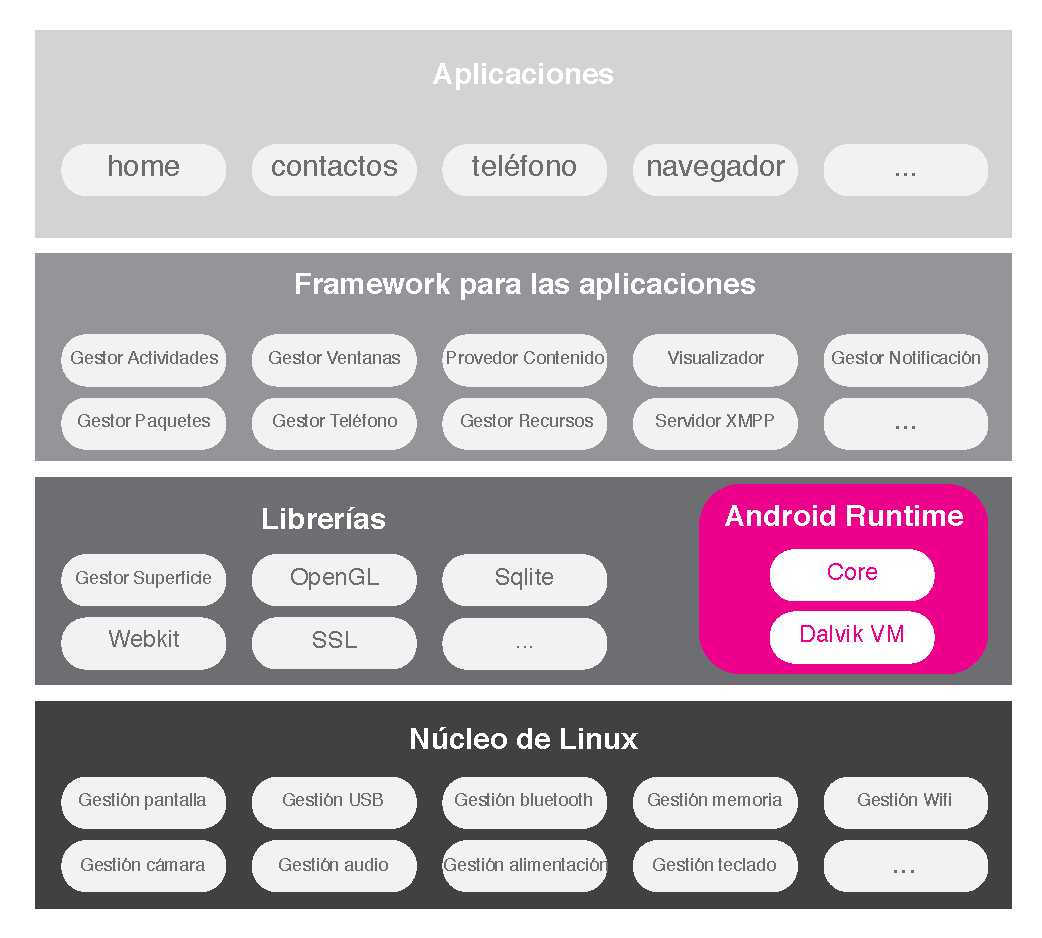
\includegraphics[scale=0.8]{./imgs/esquemas/arquitectura.pdf}
\caption{Arquitectura Android}
\label{fig:arquitectura_android}
\end{figure}

En la figura \ref{fig:arquitectura_android} vemos un esquema de la arquitectura Android, compuesta por:
\begin{itemize}
\item \emph{Núcleo Linux}: el núcleo es un fork de la versión 2.6 de Linux. Sirve de abstracción con el hardware y gestiona los recursos del sistema. 
\item \emph{Librerías}: librerías nativas del sistema las utilizará el framework de Android para comunicarse con el hardware. Están escritas en C o C++.
\item \emph{Android Runtime}: se trata del entorno de ejecución de Android. Se integra con las librerías. Aquí tenemos el conjunto de librerías habituales de java, así como librerías Java específicas para Android. La Dalvik VM, es la máquina virtual de Java que ejecutará la aplicaciones. 
\item \emph{Framework para aplicaciones}: Capa formada por las clases y servicios que utilizan directamente las aplicaciones de usuario para interactuar con Android. 
\item \emph{Aplicaciones}: esta última capa incluye todas las aplicaciones del sistema y las instaladas por el usuario, tanto las nativas como las escritas en java.

\end{itemize}




\subsection{Segmentación}
El hecho de que exista una amplia gama de dispositivos que utilizan Android como sistema operativo también tiene una parte negativa y es que los terminales más antiguos ejecutan versiones obsoletas de Android y no es posible actualizarlos. Lo que lleva a que en el mercado convivan distintas versiones de Android.\par

La segmentación es uno de los problemas con los que tiene que lidiar Android. En la actualidad conviven 7 distribuciones de Android.\par
Desde la web de Android \cite{android} mantienen una tabla con el porcentaje de dispositivos que usan cada versión (tabla \ref{android:distro}).\medskip\par

\begin{table}
\begin{center}

  
  \begin{tabular}{ |l|l|l|l| }
    \hline
    \rowcolor{RubineRed} {\color{White} Versión} & {\color{White} Nombre }& {\color{White} Nivel API }& {\color{White} Distribución} \\ \hline
    1.6 & Donut & 4 & 0.1\%  \\ \hline
    2.1 & Eclair & 7 & 1.2\%  \\ \hline
    2.2 & Froyo & 8 & 2.5\%  \\ \hline
    2.3-2.3.2 & Gingerbread & 9 & 0.1\%  \\ \hline
    2.3.3-2.3.7 & Gingerbread & 10 & 33.0\%  \\ \hline
    3.2 & Honeycomb & 13 & 0.1\%  \\ \hline
    3.2 & Ice Cream Sandwich & 15 & 22.5\%  \\ \hline
    4.1 & JellyBean & 16 & 34.0\%  \\ \hline
    4.2 & JellyBean & 17 & 6.5\%  \\ \hline
    
    \end{tabular}
\end{center}
\caption{Distribución de las versiones de la plataforma Android}
  \label{android:distro}
\end{table}

Lo que recomienda Google a la hora de seleccionar una versión de Android es que lleguemos a una solución de compromiso entre las características que necesitamos utilizar de la API y el porcentaje de dispositivos en los que nuestra aplicación se podrá instalar.\par

\subsection{Tabletas e interfaces táctiles de grandes dimensiones}
Las pantallas táctiles de los móviles facilitan la interacción con los usuarios, pero cuanto más grande son las pantallas más sencillo es el proceso. Por lo tanto planteamos este proyecto centrándonos en tabletas de al menos 10 pulgadas, y teniendo en mente dispositivos de mayores dimensiones.\medskip\par
A partir de la versión 3.2 \emph{Honeycomb}, Google hace un profundo rediseño de su plataforma para adaptarse a las tabletas y el resto de dispositivos con altas resoluciones. A partir de esta versión introducen mecanismos específicos para trabajar con pantallas más grandes.\par
Android permite establecer la versión mínima necesaria para ejecutar la aplicación (\emph{android:minSdkVersion}), en nuestro caso escogeremos \emph{Honeycomb}, pues se trata de la primera versión que soporta directamente tabletas. Sin embargo para de seleccionar la versión para la que diseñaremos la aplicación tendremos en cuenta las características que nos ofrecen \emph{Honeycomb, Ice cream y JellyBean} y el porcentaje de dispositivos que las soportan.\par

\begin{figure}[ht]
\centering
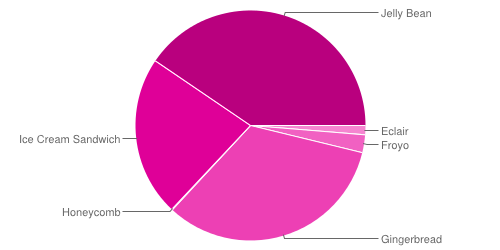
\includegraphics[scale=0.8]{./imgs/esquemas/chart.png}
\caption{Gráfico con la distribución de las versiones de la plataforma Android}
\label{fig:android_distribucion}
\end{figure}
Vemos el gráfico con la distribución de versiones de la SDK entre los dispositivos Android en la figura \ref{fig:android_distribucion}.


\begin{itemize}
  \item \emph{Honeycomb}:
    \begin{itemize} 
      \item Presenta una nueva interfaz de usuario.
      \item Gráficos acelerados por hardware.
      \item Multiselección
      \item Soportada por el 63.1\% de los dispositivos.
    \end{itemize}
    \item \emph{Ice cream Sandwich}:
    \begin{itemize} 
      \item Unificación de la interfaz de usuario.
      \item Mejora la aceleración gráfica.
      \item Mejora el soporte a múltiples pantallas. 
      \item Soportada por el 63\% de los dispositivos.
    \end{itemize}
  \item \emph{JellyBean}:
    \begin{itemize} 
      \item Simplificada la navegación.
      \item Mejora el comportamiento de los dispositivos.
      \item Mejora las notificaciones
      \item Soportada por el 40.5\% de los dispositivos.
    \end{itemize}
\end{itemize}
A la vista de esto, optamos por que la aplicación que se genera a partir de una plantilla de informe DICOM-SR fuera dirigida a Ice Cream Sandwich, puesto que ya tiene la mayor parte de las mejoras significativas de Android para tabletas y es soportada por un importante número de dispositivos.\par
Si en el futuro aparecieran mejoras que creyereamos indispensables siempre podríamos modificar las plantillas con el código  que genera la aplicación para utilizar otra versión de Android.\par


\section{Python}\label{sec:tecnologias:python}
La elección óptima de un lenguaje de programación para un proyecto determinado depende de varios factores: el equipo de desarrollo, las características del propio proyecto, las características del lenguaje\ldots\par
En este proyecto lo fundamental es la generación de código y uno de los puntos fuertes de este paradigma es que el lenguaje de programación que utilizamos para generar la aplicación y el lenguaje de la propia aplicación no tienen porque coincidir. En nuestro caso el lenguaje de la aplicación viene fijado por el problema que queremos resolver. Sin embargo podremos elegir el lenguaje para generar el código que más se adapte a nuestras necesidades.\par
Las características que debe tener un lenguaje de programación para ser apropiado para la generación de código son las siguientes \cite{herrington2003code}:
\begin{itemize}
\item Deben ser muy eficientes en la lectura, análisis gramatical y escritura de texto.
\item Deben disponer de mecanismos para crear plantillas de texto fácilmente.
\item Si soportan de manera nativa XML es útil aunque siempre se pueden incluir librerías externas para leer y manipular XML.
\item Deben ser multiplataforma.
\item La velocidad de ejecución del lenguaje no es un punto clave porque se ejecutará en producción. Es la aplicación que genere la que debe tener un buen rendimiento.
\item Su desarrollo y mantenimiento debe ser sencillo. 
\end{itemize}
\medskip\par
Pensando en todos estos puntos decidimos utilizar Python como lenguaje para generar el código de la aplicación Android.\par
Python es un lenguaje de alto nivel multipropósito y multiplataforma diseñado por Guido van Rossum en 1991. Es un lenguaje que fomenta la escritura de código legible con una sintaxis sencilla. Por su simplicidad muchas veces se utiliza como un lenguaje de scripting pero es un lenguaje suficientemente potente para utilizarlo en otros muchos contextos.\par
La implementación más común de Python esta escrita en C, se trata de CPython. Es una implementación de código abierto y gratuita, gestionada por la asociación sin ánimo de lucro  de Python (\emph{Python Software Foundation}) \cite{python}.\medskip\par
Uno de los puntos fuertes de este lenguaje es su amplia librería estándar que nos permite hacer análisis sintáctico, acceder a la API de XML, utilizar expresiones regulares, hacer uso de plantillas,\ldots de manera simple.\par
Es especialmente apropiado para este problema porque cumple todas las premisas que debe tener un buen lenguaje para la generación de código.\par
En 2009 Python lanzó su versión 3.0, la primera versión no compatible con las versiones anteriores. A pesar de que introduce un buen número de mejoras, algunas librerías externas todavía no son compatibles con esta versión. Por esto para este proyecto utilizaremos la versión 2.7 de Python. Aunque existen mecanismos \cite{py:2to3} para portar automáticamente una aplicación de Python 2.x a Python 3.x.\par
En este proyecto haremos uso de un paradigma de programación orientado a objetos, así como de las librerías estándar para gestionar la configuración, el análisis sintáctico y la parte más sencilla de las plantillas. La única librería externa que utilizaremos será Jinja, para la gestión de plantillas más complejas. Hablaremos en detalle de esto en los apartados \ref{req:implementacion}, \ref{sec:configuracion} y \ref{sec:templates}.



\chapter{Desarrollo}
\section{Análisis de los requisitos}
\section{Diseño}
\section{Implementación}
\section{Verificación: un caso práctico}

\chapter{Conclusiones}

\chapter{Futuras mejoras}

%\printbibliography
\bibliographystyle{unsrtnat}
\bibliography{bibliografia}

\appendix
\chapter{Informe DICOM-SR}\label{dicom-sr}
\lstset{escapechar=@,style=dicom}
\renewcommand*\lstlistingname{Fichero}

\begin{lstlisting}[label=dicom-report,caption=Informe estructurado de una exploración de mama]

<?xml version="1.0" encoding="ISO-8859-1"?>

<!-- DICOM HEADER -->

<DICOM_SR Description="Exploration of breast" IDOntology="4">
  <CONTAINER>
    <CONCEPT_NAME>
      <CODE_VALUE>172117008</CODE_VALUE>
      <CODE_SCHEMA>SNOMED-CT</CODE_SCHEMA>
      <CODE_MEANING>Exploration of Breast</CODE_MEANING>
    </CONCEPT_NAME>
    <CHILDS>
      <DATE>
        <CONCEPT_NAME>
          <CODE_VALUE>399651003</CODE_VALUE>
          <CODE_SCHEMA>SNOMED-CT</CODE_SCHEMA>
          <CODE_MEANING>Date of Report</CODE_MEANING>
        </CONCEPT_NAME>
        <VALUE> 28-07-2007 </VALUE>
      </DATE>
      <NUM>
        <CONCEPT_NAME>
          <CODE_VALUE>118522005</CODE_VALUE>
          <CODE_SCHEMA>SNOMED-CT</CODE_SCHEMA>
          <CODE_MEANING>Identifier</CODE_MEANING>
        </CONCEPT_NAME>
        <VALUE> 1234ABC </VALUE>
      </NUM>
      <NUM>
        <CONCEPT_NAME>
          <CODE_VALUE>RID13159</CODE_VALUE>
          <CODE_SCHEMA>RADLEX</CODE_SCHEMA>
          <CODE_MEANING>Patient Identifier</CODE_MEANING>
        </CONCEPT_NAME>
        <VALUE> 12345678X </VALUE>
      </NUM>

      <!-- RIGHT FEMALE BREAST -->
      <CONTAINER>
        <CONCEPT_NAME>
         <CODE_VALUE>RID29896</CODE_VALUE>
         <CODE_SCHEMA>RADLEX</CODE_SCHEMA>
         <CODE_MEANING>Right Female Breast</CODE_MEANING>
        </CONCEPT_NAME>

        <!-- RIGHT FEMALE BREAST INJURIES -->
        <CHILDS>
          <CONTAINER>
            <CONCEPT_NAME>
              <CODE_VALUE>RID3874</CODE_VALUE>
              <CODE_SCHEMA>RADLEX</CODE_SCHEMA>
              <CODE_MEANING>Mass</CODE_MEANING>
            </CONCEPT_NAME>
            <CHILDS>
              <TEXT>
                <CONCEPT_NAME>
                  <CODE_VALUE>118522005</CODE_VALUE>
                  <CODE_SCHEMA>SNOMED-CT</CODE_SCHEMA>
                  <CODE_MEANING>Identifier</CODE_MEANING>
                </CONCEPT_NAME>
                <VALUE> M001 </VALUE>
              </TEXT>
              <NUM>
                <CONCEPT_NAME>
                  <CODE_VALUE>RID29929</CODE_VALUE>
                  <CODE_SCHEMA>RADLEX</CODE_SCHEMA>
                  <CODE_MEANING>Upper Outer Quadrant of Right Female Breast</CODE_MEANING>
                </CONCEPT_NAME>
                <VALUE> TRUE </VALUE>
              </NUM>
              <NUM>
                <CONCEPT_NAME>
                  <CODE_VALUE>RID29935</CODE_VALUE>
                  <CODE_SCHEMA>RADLEX</CODE_SCHEMA>
                  <CODE_MEANING>Lower Outer Quadrant of Right Female Breast</CODE_MEANING>
                </CONCEPT_NAME>
                <VALUE> TRUE </VALUE>
              </NUM>
              <NUM>
                <CONCEPT_NAME>
                  <CODE_VALUE>RID29934</CODE_VALUE>
                  <CODE_SCHEMA>RADLEX</CODE_SCHEMA>
                  <CODE_MEANING>Lower Outer Quadrant of Breast</CODE_MEANING>
                </CONCEPT_NAME>
                <VALUE> FALSE </VALUE>
              </NUM>
              <NUM>
                <CONCEPT_NAME>
                  <CODE_VALUE>RID29932</CODE_VALUE>
                  <CODE_SCHEMA>RADLEX</CODE_SCHEMA>
                  <CODE_MEANING>Upper Inner Quadrant of Right Female Breast</CODE_MEANING>
                </CONCEPT_NAME>
                <VALUE> FALSE </VALUE>
              </NUM>
              <NUM>
                <CONCEPT_NAME>
                  <CODE_VALUE>RID29938</CODE_VALUE>
                  <CODE_SCHEMA>RADLEX</CODE_SCHEMA>
                  <CODE_MEANING>Lower Inner Quadrant of Right Female Breast</CODE_MEANING>
                </CONCEPT_NAME>
                <VALUE> FALSE </VALUE>
              </NUM>
              <NUM>
                <CONCEPT_NAME>
                  <CODE_VALUE>RID29947</CODE_VALUE>
                  <CODE_SCHEMA>RADLEX</CODE_SCHEMA>
                  <CODE_MEANING>Lateral Region of Right Female Breast</CODE_MEANING>
                </CONCEPT_NAME>
                <VALUE> FALSE </VALUE>
              </NUM>
              <NUM>
                <CONCEPT_NAME>
                  <CODE_VALUE>RID29941</CODE_VALUE>
                  <CODE_SCHEMA>RADLEX</CODE_SCHEMA>
                  <CODE_MEANING>Superior Region of Right Female Breast</CODE_MEANING>
                </CONCEPT_NAME>
                <VALUE> TRUE </VALUE>
              </NUM>
              <NUM>
                <CONCEPT_NAME>
                  <CODE_VALUE>RID29953</CODE_VALUE>
                  <CODE_SCHEMA>RADLEX</CODE_SCHEMA>
                  <CODE_MEANING>Subareolar Region of  Right Female Breast</CODE_MEANING>
                </CONCEPT_NAME>
                <VALUE> FALSE </VALUE>
              </NUM>
              <NUM>
                <CONCEPT_NAME>
                  <CODE_VALUE>RID29944</CODE_VALUE>
                  <CODE_SCHEMA>RADLEX</CODE_SCHEMA>
                  <CODE_MEANING>Medial Region of Right Breast</CODE_MEANING>
                </CONCEPT_NAME>
                <VALUE> FALSE </VALUE>
              </NUM>
              <NUM>	
                <CONCEPT_NAME>
                  <CODE_VALUE>RID29950</CODE_VALUE>
                  <CODE_SCHEMA>RADLEX</CODE_SCHEMA>
                  <CODE_MEANING>Central Region of Right Breast</CODE_MEANING>
                </CONCEPT_NAME>
                <VALUE> FALSE </VALUE>
              </NUM>
              <NUM>
                <CONCEPT_NAME>
                  <CODE_VALUE>RID29907</CODE_VALUE>
                  <CODE_SCHEMA>RADLEX</CODE_SCHEMA>
                  <CODE_MEANING>Nipple of Right Female Breast</CODE_MEANING>
                </CONCEPT_NAME>
                <VALUE> FALSE </VALUE>
              </NUM>
              <NUM>
                <CONCEPT_NAME>
                  <CODE_VALUE>RID29918</CODE_VALUE>
                  <CODE_SCHEMA>RADLEX</CODE_SCHEMA>
                  <CODE_MEANING>Areola of Right Female Breast</CODE_MEANING>
                </CONCEPT_NAME>
                <VALUE> FALSE </VALUE>
              </NUM>
              <NUM>
                <CONCEPT_NAME>
                  <CODE_VALUE>TRMM0001</CODE_VALUE>
                  <CODE_SCHEMA>TRENCADIS_MAMO</CODE_SCHEMA>
                  <CODE_MEANING>Axillary Tail of Right Female Breast</CODE_MEANING>
                </CONCEPT_NAME>
                <VALUE> FALSE </VALUE>
              </NUM>
              <NUM>
                <CONCEPT_NAME>
                  <CODE_VALUE>TRMM0003</CODE_VALUE>
                  <CODE_SCHEMA>TRENCADIS_MAMO</CODE_SCHEMA>
                  <CODE_MEANING>Axillary Region of Right Female Breast</CODE_MEANING>
                </CONCEPT_NAME>
                <VALUE> FALSE </VALUE>
              </NUM>
              <NUM>
                <CONCEPT_NAME>
                  <CODE_VALUE>TRMM0005</CODE_VALUE>
                  <CODE_SCHEMA>TRENCADIS_MAMO</CODE_SCHEMA>
                  <CODE_MEANING>Inframammary Sulcus of Right Female Breast</CODE_MEANING>
                </CONCEPT_NAME>
              </NUM>
              <NUM>
                <CONCEPT_NAME>
                  <CODE_VALUE>TRMM0007</CODE_VALUE>
                  <CODE_SCHEMA>TRENCADIS_MAMO</CODE_SCHEMA>
                  <CODE_MEANING>Intermammary Sulcus of Right Female Breast</CODE_MEANING>
                </CONCEPT_NAME>
              </NUM>
            </CHILDS>
      </CONTAINER>

      <!-- LEFT FEMALE BREAST -->
      <CONTAINER>
        <CONCEPT_NAME>
         <CODE_VALUE>RID29897</CODE_VALUE>
         <CODE_SCHEMA>RADLEX</CODE_SCHEMA>
         <CODE_MEANING>Left Female Breast</CODE_MEANING>
        </CONCEPT_NAME>

        <!-- LEFT FEMALE BREAST INJURIES -->
        <CHILDS>
          <CONTAINER>
            <CONCEPT_NAME>
              <CODE_VALUE>RID34265</CODE_VALUE>
              <CODE_SCHEMA>RADLEX</CODE_SCHEMA>
              <CODE_MEANING>Asymmetry</CODE_MEANING>
            </CONCEPT_NAME>
            <CHILDS>
              <TEXT>
                <CONCEPT_NAME>
                  <CODE_VALUE>118522005</CODE_VALUE>
                  <CODE_SCHEMA>SNOMED-CT</CODE_SCHEMA>
                  <CODE_MEANING>Identifier</CODE_MEANING>
                </CONCEPT_NAME>
                <VALUE> A001 </VALUE>
              </TEXT>
              <NUM>
                <CONCEPT_NAME>
                  <CODE_VALUE>RID29930</CODE_VALUE>
                  <CODE_SCHEMA>RADLEX</CODE_SCHEMA>
                  <CODE_MEANING>Upper Outer Quadrant of Left Female Breast</CODE_MEANING>
                </CONCEPT_NAME>
                <VALUE> FALSE </VALUE>
              </NUM>
              <NUM>
                <CONCEPT_NAME>
                  <CODE_VALUE>RID29936</CODE_VALUE>
                  <CODE_SCHEMA>RADLEX</CODE_SCHEMA>
                  <CODE_MEANING>Lower Outer Quadrant of Left Female Breast</CODE_MEANING>
                <VALUE> FALSE </VALUE>
              </NUM>
              <NUM>
                <CONCEPT_NAME>
                  <CODE_VALUE>RID29933</CODE_VALUE>
                  <CODE_SCHEMA>RADLEX</CODE_SCHEMA>
                  <CODE_MEANING>Upper Inner Quadrant of Left Female Breast</CODE_MEANING>
                </CONCEPT_NAME>
                <VALUE> FALSE </VALUE>
              </NUM>
              <NUM>
                <CONCEPT_NAME>
                  <CODE_VALUE>RID29939</CODE_VALUE>
                  <CODE_SCHEMA>RADLEX</CODE_SCHEMA>
                  <CODE_MEANING>Lower Inner Quadrant of Left Female Breast</CODE_MEANING>
                </CONCEPT_NAME>
                <VALUE> FALSE </VALUE>
              </NUM>
              <NUM>
                <CONCEPT_NAME>
                  <CODE_VALUE>RID29948</CODE_VALUE>
                  <CODE_SCHEMA>RADLEX</CODE_SCHEMA>
                  <CODE_MEANING>Lateral Region of Left Breast</CODE_MEANING>
                </CONCEPT_NAME>
                <VALUE> TRUE </VALUE>
              </NUM>
              <NUM>
                <CONCEPT_NAME>
                  <CODE_VALUE>RID29942</CODE_VALUE>
                  <CODE_SCHEMA>RADLEX</CODE_SCHEMA>
                  <CODE_MEANING>Superior Region of Left Breast</CODE_MEANING>
                </CONCEPT_NAME>
                <VALUE> TRUE </VALUE>
              </NUM>
              <NUM>
                <CONCEPT_NAME>
                  <CODE_VALUE>RID29954</CODE_VALUE>
                  <CODE_SCHEMA>RADLEX</CODE_SCHEMA>
                  <CODE_MEANING>Subareolar Region of Left Breast</CODE_MEANING>
                </CONCEPT_NAME>
                <VALUE> FALSE </VALUE>
              </NUM>
              <NUM>
                <CONCEPT_NAME>
                  <CODE_VALUE>RID29945</CODE_VALUE>
                  <CODE_SCHEMA>RADLEX</CODE_SCHEMA>
                  <CODE_MEANING>Medial Region of Left Breast</CODE_MEANING>
                </CONCEPT_NAME>
                <VALUE> FALSE </VALUE>
              </NUM>
              <NUM>
                <CONCEPT_NAME>
                  <CODE_VALUE>RID29951</CODE_VALUE>
                  <CODE_SCHEMA>RADLEX</CODE_SCHEMA>
                  <CODE_MEANING>Central Region of Left Breast</CODE_MEANING>
                </CONCEPT_NAME>
                <VALUE> FALSE </VALUE>
              </NUM>
              <NUM>
                <CONCEPT_NAME>
                  <CODE_VALUE>RID29908</CODE_VALUE>
                  <CODE_SCHEMA>RADLEX</CODE_SCHEMA>
                  <CODE_MEANING>Nipple of Left Female Breast</CODE_MEANING>
                </CONCEPT_NAME>
                <VALUE> FALSE </VALUE>
              </NUM>
              <NUM>
                <CONCEPT_NAME>
                  <CODE_VALUE>RID29919</CODE_VALUE>
                  <CODE_SCHEMA>RADLEX</CODE_SCHEMA>
                  <CODE_MEANING>Areola of Left Female Breast</CODE_MEANING>
                </CONCEPT_NAME>
                <VALUE> FALSE </VALUE>
              </NUM>
              <NUM>
                <CONCEPT_NAME>
                  <CODE_VALUE>TRMM0002</CODE_VALUE>
                  <CODE_SCHEMA>TRENCADIS_MAMO</CODE_SCHEMA>
                  <CODE_MEANING>Axillary Tail of Left Female Breast</CODE_MEANING>
                </CONCEPT_NAME>
                <VALUE> FALSE </VALUE>
              </NUM>
              <NUM>
              <CONCEPT_NAME>
                <CODE_VALUE>TRMM0004</CODE_VALUE>
                <CODE_SCHEMA>TRENCADIS_MAMO</CODE_SCHEMA>
                  <CODE_MEANING>Axillary Region of Left Female Breast</CODE_MEANING>
                </CONCEPT_NAME>
                <VALUE> FALSE </VALUE>
              </NUM>
              <NUM>
                <CONCEPT_NAME>
                  <CODE_VALUE>TRMM0006</CODE_VALUE>
                  <CODE_SCHEMA>TRENCADIS_MAMO</CODE_SCHEMA>
                  <CODE_MEANING>Inframammary Sulcus  of Left Female Breast</CODE_MEANING>
                </CONCEPT_NAME>
                <VALUE> FALSE </VALUE>
              </NUM>
              <NUM>
                <CONCEPT_NAME>
                  <CODE_VALUE>TRMM0008</CODE_VALUE>
                  <CODE_SCHEMA>TRENCADIS_MAMO</CODE_SCHEMA>
                  <CODE_MEANING>Intermammary Sulcus  of Left Female Breast</CODE_MEANING>
                </CONCEPT_NAME>
                <VALUE> FALSE </VALUE>
              </NUM>
            </CHILDS>
          </CONTAINER>
          <CONTAINER>
            <CONCEPT_NAME>
              <CODE_VALUE>RID34265</CODE_VALUE>
              <CODE_SCHEMA>RADLEX</CODE_SCHEMA>
              <CODE_MEANING>Asymmetry</CODE_MEANING>
            </CONCEPT_NAME>
            <CHILDS>
              <TEXT>
                <CONCEPT_NAME>
                  <CODE_VALUE>118522005</CODE_VALUE>
                  <CODE_SCHEMA>SNOMED-CT</CODE_SCHEMA>
                  <CODE_MEANING>Identifier</CODE_MEANING>
                </CONCEPT_NAME>
                <VALUE> A002 </VALUE>
              </TEXT>
              <NUM>
                <CONCEPT_NAME>
                  <CODE_VALUE>RID29930</CODE_VALUE>
                  <CODE_SCHEMA>RADLEX</CODE_SCHEMA>
                  <CODE_MEANING>Upper Outer Quadrant of Left Female Breast</CODE_MEANING>
                </CONCEPT_NAME>
                <VALUE> FALSE </VALUE>
              </NUM>
              <NUM>
                <CONCEPT_NAME>
                  <CODE_VALUE>RID29936</CODE_VALUE>
                  <CODE_SCHEMA>RADLEX</CODE_SCHEMA>
                  <CODE_MEANING>Lower Outer Quadrant of Left Female Breast</CODE_MEANING>
                <VALUE> FALSE </VALUE>
              </NUM>
              <NUM>
                <CONCEPT_NAME>
                  <CODE_VALUE>RID29933</CODE_VALUE>
                  <CODE_SCHEMA>RADLEX</CODE_SCHEMA>
                  <CODE_MEANING>Upper Inner Quadrant of Left Female Breast</CODE_MEANING>
                </CONCEPT_NAME>
                <VALUE> FALSE </VALUE>
              </NUM>
              <NUM>
                <CONCEPT_NAME>
                  <CODE_VALUE>RID29939</CODE_VALUE>
                  <CODE_SCHEMA>RADLEX</CODE_SCHEMA>
                  <CODE_MEANING>Lower Inner Quadrant of Left Female Breast</CODE_MEANING>
                </CONCEPT_NAME>
                <VALUE> FALSE </VALUE>
              </NUM>
              <NUM>
                <CONCEPT_NAME>
                  <CODE_VALUE>RID29948</CODE_VALUE>
                  <CODE_SCHEMA>RADLEX</CODE_SCHEMA>
                  <CODE_MEANING>Lateral Region of Left Breast</CODE_MEANING>
                </CONCEPT_NAME>
                <VALUE> FALSE </VALUE>
              </NUM>
              <NUM>
                <CONCEPT_NAME>
                  <CODE_VALUE>RID29942</CODE_VALUE>
                  <CODE_SCHEMA>RADLEX</CODE_SCHEMA>
                  <CODE_MEANING>Superior Region of Left Breast</CODE_MEANING>
                </CONCEPT_NAME>
                <VALUE> FALSE </VALUE>
              </NUM>
              <NUM>
                <CONCEPT_NAME>
                  <CODE_VALUE>RID29954</CODE_VALUE>
                  <CODE_SCHEMA>RADLEX</CODE_SCHEMA>
                  <CODE_MEANING>Subareolar Region of Left Breast</CODE_MEANING>
                </CONCEPT_NAME>
                <VALUE> FALSE </VALUE>
              </NUM>
              <NUM>
                <CONCEPT_NAME>
                  <CODE_VALUE>RID29945</CODE_VALUE>
                  <CODE_SCHEMA>RADLEX</CODE_SCHEMA>
                  <CODE_MEANING>Medial Region of Left Breast</CODE_MEANING>
                </CONCEPT_NAME>
                <VALUE> FALSE </VALUE>
              </NUM>
              <NUM>
                <CONCEPT_NAME>
                  <CODE_VALUE>RID29951</CODE_VALUE>
                  <CODE_SCHEMA>RADLEX</CODE_SCHEMA>
                  <CODE_MEANING>Central Region of Left Breast</CODE_MEANING>
                </CONCEPT_NAME>
                <VALUE> FALSE </VALUE>
              </NUM>
              <NUM>
                <CONCEPT_NAME>
                  <CODE_VALUE>RID29908</CODE_VALUE>
                  <CODE_SCHEMA>RADLEX</CODE_SCHEMA>
                  <CODE_MEANING>Nipple of Left Female Breast</CODE_MEANING>
                </CONCEPT_NAME>
                <VALUE> FALSE </VALUE>
              </NUM>
              <NUM>
                <CONCEPT_NAME>
                  <CODE_VALUE>RID29919</CODE_VALUE>
                  <CODE_SCHEMA>RADLEX</CODE_SCHEMA>
                  <CODE_MEANING>Areola of Left Female Breast</CODE_MEANING>
                </CONCEPT_NAME>
                <VALUE> FALSE </VALUE>
              </NUM>
              <NUM>
                <CONCEPT_NAME>
                  <CODE_VALUE>TRMM0002</CODE_VALUE>
                  <CODE_SCHEMA>TRENCADIS_MAMO</CODE_SCHEMA>
                  <CODE_MEANING>Axillary Tail of Left Female Breast</CODE_MEANING>
                </CONCEPT_NAME>
                <VALUE> TRUE </VALUE>
              </NUM>
              <NUM>
              <CONCEPT_NAME>
                <CODE_VALUE>TRMM0004</CODE_VALUE>
                <CODE_SCHEMA>TRENCADIS_MAMO</CODE_SCHEMA>
                  <CODE_MEANING>Axillary Region of Left Female Breast</CODE_MEANING>
                </CONCEPT_NAME>
                <VALUE> FALSE </VALUE>
              </NUM>
              <NUM>
                <CONCEPT_NAME>
                  <CODE_VALUE>TRMM0006</CODE_VALUE>
                  <CODE_SCHEMA>TRENCADIS_MAMO</CODE_SCHEMA>
                  <CODE_MEANING>Inframammary Sulcus  of Left Female Breast</CODE_MEANING>
                </CONCEPT_NAME>
                <VALUE> FALSE </VALUE>
              </NUM>
              <NUM>
                <CONCEPT_NAME>
                  <CODE_VALUE>TRMM0008</CODE_VALUE>
                  <CODE_SCHEMA>TRENCADIS_MAMO</CODE_SCHEMA>
                  <CODE_MEANING>Intermammary Sulcus  of Left Female Breast</CODE_MEANING>
                </CONCEPT_NAME>
                <VALUE> FALSE </VALUE>
              </NUM>
            </CHILDS>
          </CONTAINER>
        </CHILDS>
      </CONTAINER>
    </CHILDS>
  </CONTAINER>
<DICOM_SR>

\end{lstlisting}

\chapter{Plantilla de un informe DICOM-SR}\label{dicom-sr-template}


\end{document}